\documentclass[a4paper,11pt]{scrartcl}%scrbook %[...,twoside]

\usepackage[a4paper,left=3.5cm,right=2.5cm,bottom=3.5cm,top=3cm]{geometry}

\usepackage[ngerman]{babel}

% Caption Packet
\usepackage[margin=0pt,font=small,labelfont=bf]{caption}
% Gliederung einstellen
\setcounter{secnumdepth}{5}
%\setcounter{tocdepth}{5}
%\usepackage[Sonny]{fncychap}
%\ChTitleVar{\huge\rm}
\usepackage[pdftex]{graphicx,color}
\usepackage{amsmath,amssymb}
% Theorem-Umgebungen
\usepackage[amsmath,thmmarks]{ntheorem}
% Korrekte Darstellung der Umlaute
\usepackage[utf8]{inputenc}
\usepackage[T1]{fontenc}
\usepackage{lmodern}
\usepackage[onehalfspacing]{setspace}
% Algorithmen
 \usepackage[linesnumbered,ruled,vlined]{algorithm2e}
\usepackage{algorithmic}
%\renewcommand{\algorithmiccomment}[1]{\hfill \tiny//~#1\normalsize}
% Bibtex deutsch
\usepackage{bibgerm}
% URLs
\usepackage{url}
\usepackage{verbatim}

% Theorem-Optionen %
\theoremseparator{}
\theoremstyle{change}
\newtheorem{theorem}{Theorem}[section]
\newtheorem{satz}[theorem]{Satz}
\newtheorem{lemma}[theorem]{Lemma}
\newtheorem{korollar}[theorem]{Korollar}
\newtheorem{proposition}[theorem]{Proposition}
% Ohne Numerierung
\theoremstyle{nonumberplain}
\renewtheorem{theorem*}{Theorem}
\renewtheorem{satz*}{Satz}
\renewtheorem{lemma*}{Lemma}
\renewtheorem{korollar*}{Korollar}
\renewtheorem{proposition*}{Proposition}
% Definitionen mit \upshape
\theorembodyfont{\upshape}
\theoremstyle{change}
\newtheorem{definition}[theorem]{Definition}
\theoremstyle{nonumberplain}
\renewtheorem{definition*}{Definition}
% Kursive Schrift
\theoremheaderfont{\itshape}
\newtheorem{notation}{Notation}
\newtheorem{konvention}{Konvention}
\newtheorem{bezeichnung}{Bezeichnung}
\theoremsymbol{\ensuremath{\Box}}
\newtheorem{beweis}{Beweis}
\theoremsymbol{}
\theoremstyle{change}
\theoremheaderfont{\bfseries}
\newtheorem{bemerkung}[theorem]{Bemerkung}
\newtheorem{beobachtung}[theorem]{Beobachtung}
\newtheorem{beispiel}[theorem]{Beispiel}
\newtheorem{problem}{Problem}
\theoremstyle{nonumberplain}
\renewtheorem{bemerkung*}{Bemerkung}
\renewtheorem{beispiel*}{Beispiel}
\renewtheorem{problem*}{Problem}
%
%% Algorithmen anpassen %
%\renewcommand{\algorithmicrequire}{\textit{Eingabe:}}
%\renewcommand{\algorithmicensure}{\textit{Ausgabe:}}
%\floatname{algorithm}{Algorithmus}
%\renewcommand{\listalgorithmname}{Algorithmenverzeichnis}
%\renewcommand{\algorithmiccomment}[1]{\color{grau}{// #1}}
%
% Floating-Umgebungen anpassen %
\renewcommand{\topfraction}{0.9}
\renewcommand{\bottomfraction}{0.8}
% Abkuerzungen richtig formatieren %
\usepackage{xspace}
\newcommand{\vgl}{vgl.\@\xspace} 
\newcommand{\zB}{z.\nolinebreak[4]\hspace{0.125em}\nolinebreak[4]B.\@\xspace}
\newcommand{\bzw}{bzw.\@\xspace}
\newcommand{\dahe}{d.\nolinebreak[4]\hspace{0.125em}h.\nolinebreak[4]\@\xspace}
\newcommand{\etc}{etc.\@\xspace}
\newcommand{\evtl}{evtl.\@\xspace}
\newcommand{\ggf}{ggf.\@\xspace}
\newcommand{\bzgl}{bzgl.\@\xspace}
\newcommand{\so}{s.\nolinebreak[4]\hspace{0.125em}\nolinebreak[4]o.\@\xspace}
\newcommand{\iA}{i.\nolinebreak[4]\hspace{0.125em}\nolinebreak[4]A.\@\xspace}
\newcommand{\sa}{s.\nolinebreak[4]\hspace{0.125em}\nolinebreak[4]a.\@\xspace}
\newcommand{\su}{s.\nolinebreak[4]\hspace{0.125em}\nolinebreak[4]u.\@\xspace}
\newcommand{\ua}{u.\nolinebreak[4]\hspace{0.125em}\nolinebreak[4]a.\@\xspace}
\newcommand{\og}{o.\nolinebreak[4]\hspace{0.125em}\nolinebreak[4]g.\@\xspace}
\newcommand{\oBdA}{o.\nolinebreak[4]\hspace{0.125em}\nolinebreak[4]B.\nolinebreak[4]\hspace{0.125em}d.\nolinebreak[4]\hspace{0.125em}A.\@\xspace}
\newcommand{\OBdA}{O.\nolinebreak[4]\hspace{0.125em}\nolinebreak[4]B.\nolinebreak[4]\hspace{0.125em}d.\nolinebreak[4]\hspace{0.125em}A.\@\xspace}

\newcommand{\executeiffilenewer}[3]{%
\ifnum\pdfstrcmp{\pdffilemoddate{#1}}%
{\pdffilemoddate{#2}}>0%
{\immediate\write18{#3}}\fi%
}
% includesvg[scale]{file} command (linux-version)
\newcommand{\includesvg}[2][1]{%
  \executeiffilenewer{#2.svg}{#2.pdf}{%
  /usr/bin/inkscape -z -D --file="#2.svg" --export-pdf="#2.pdf" --export-latex}%
  \scalebox{#1}{\input{#2.pdf_tex}}%
}


% Leere Seite ohne Seitennummer, naechste Seite rechts
\newcommand{\blankpage}{
 \clearpage{\pagestyle{empty}\cleardoublepage}
}
\bibliographystyle{unsrt}
\usepackage{hyperref}
\usepackage{multirow}
% Keine einzelnen Zeilen beim Anfang eines Abschnitts (Schusterjungen)
\clubpenalty = 10000
% Keine einzelnen Zeilen am Ende eines Abschnitts (Hurenkinder)
\widowpenalty = 10000 \displaywidowpenalty = 10000
% EOF

\usepackage{tikz}
\usepackage{pgfplots}

\usepackage{hyperref}

\begin{document}
\begin{titlepage}
\definecolor{TUGreen}{rgb}{0.517,0.721,0.094}
\vspace*{-2cm}
\newlength{\links}
\setlength{\links}{-1.5cm}
\sffamily
\hspace*{\links}
\begin{minipage}{12.5cm}

\includegraphics[width=8cm]{pics/tud_logo_rgb}
%\hspace*{-0.25cm} \textbf{TECHNISCHE UNIVERSIT"AT DORTMUND}\\
%\hspace*{-1.2cm} \rule{5mm}{5mm} \hspace*{0.1cm} FACHBEREICH INFORMATIK\\
\end{minipage}

\vspace*{4cm}

\hspace*{\links}
\hspace*{-0.2cm}
\begin{minipage}{9cm}
\large
\begin{center}
{\Large Bachelorarbeit} \\
\vspace*{1cm}
\textbf{Textkompression mithilfe einer Variante von LZ78} \\
\vspace*{1cm}
Florian Kleine\\
% \vspace*{1cm}
Oktober 2016
\end{center}
\end{minipage}
\normalsize
\vspace*{5.5cm}

% \hspace*{\links}

\vspace*{2.1cm}

\hspace*{\links}
\begin{minipage}[b]{5cm}
% \normalsize
\raggedright
Gutachter: \\
Prof. Dr. Johannes Fischer \\
Dominik Köppl \\
\end{minipage}

\vspace*{2.5cm}
\hspace*{\links}
\begin{minipage}[b]{8cm}
% \normalsize
\raggedright
Technische Universit"at Dortmund \\
Fakult"at f"ur Informatik\\
Lehrstuhl für Algorithm Engineering (LS11)\\
http://ls11-www.cs.tu-dortmund.de
\end{minipage}

\end{titlepage}

\thispagestyle{empty}
\newpage
\tableofcontents
\newpage
\newpage

\section{Einleitung}
Die Datenkompression spielt in der Informatik eine große Rolle. Zwar sind die Datenträger im Vergleich zu früher um ein Vielfaches größer und vor allem günstiger geworden, stoßen bei den heute anfallenden riesigen Datenmengen aber immer noch an ihre Grenzen. Deshalb ist es sinnvoll die Daten mit geschickten Verfahren so zu komprimieren, dass sie später verlustfrei in den Ursprungszustand zurückübersetzt werden können.
In dieser Arbeit soll es darum gehen, Texte mithilfe einer Variante des Lempel-Ziv78-Verfahrens in Faktoren zu zerlegen, zu kodieren und so verlustfrei zu komprimieren. Dieses Verfahren stützt sich auf der Eliminierung von Redundanzen, indem Teile des Textes durch Verweise auf vorher auftretende gleiche Teile ersetzt werden. Solche Verweise benötigen weniger Speicher als der Text, was so zu einer Kompression des kompletten Textes führt.
Das aus dieser Arbeit entstehende Verfahren wird anschließend mit bereits vorhandenen Kompressionsverfahren (z.B. gzip und 7zip) verglichen.\\\\

\subsection{Anekdote}
Um die Bedeutung von Datenkompression zu verdeutlichen und zu zeigen, wie lange man sich über dieses Thema schon Gedanken macht, hier eine kleinen Anekdote:\\
Ende des 18. Jahrhunderts benötigte die britische Marine eine schnelle Kommunikation zwischen London und dem Marinestützpunkt an der Küste. Dies wurde durch eine Kette von Hütten auf Hügeln in etwa 5 Meilen Entfernung umgesetzt. Diese Hütten(sog. \textit{Klappentelegraphen}, \autoref{fig:braille}) hatten 6 Klappen auf dem Dach, die entweder geschlossen oder geöffnet waren. Durch diese 64 möglichen Kombinationen von offenen und geschlossenen Klappen konnte man Buchstanden des Braille-Alphabets (s. \autoref{fig:braille}) darstellen. Da das Alphabet weniger als 64 Buchstaben hat, gab es freie Kombinationen von Klappenstellungen. Diese freien Kombinationen wurden dazu benutzt die Kommunikation zu beschleunigen. Oft benutzen Wörtern wie 'for' oder 'the' wurden freie Kombinationen zugewiesen. Anderen Worten wie 'father' oder 'mother' wurde die freie Kombination 'dot5' und die Kombination für 'f' bzw. 'm' zugewiesen. So erreichte man eine Kompression von 20\% bei englischen Texten.\cite[S.1-4]{bellTextCompression} \\
Dieses Problem hat sich bis heute nicht geändert. Wie verringern wir die Datenmenge möglichst stark und beschleunigen somit die Übertragung, ohne Informationen zu verlieren?
	\begin{figure}[h]
	
		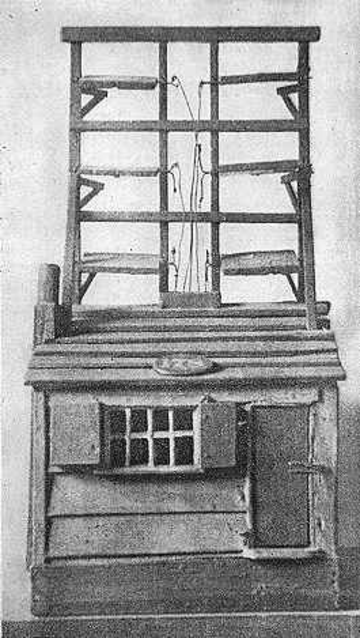
\includegraphics[scale=0.25]{./pics/shuttercabin}\cite{klappentelegraph}
		\hspace{25pt}
	 	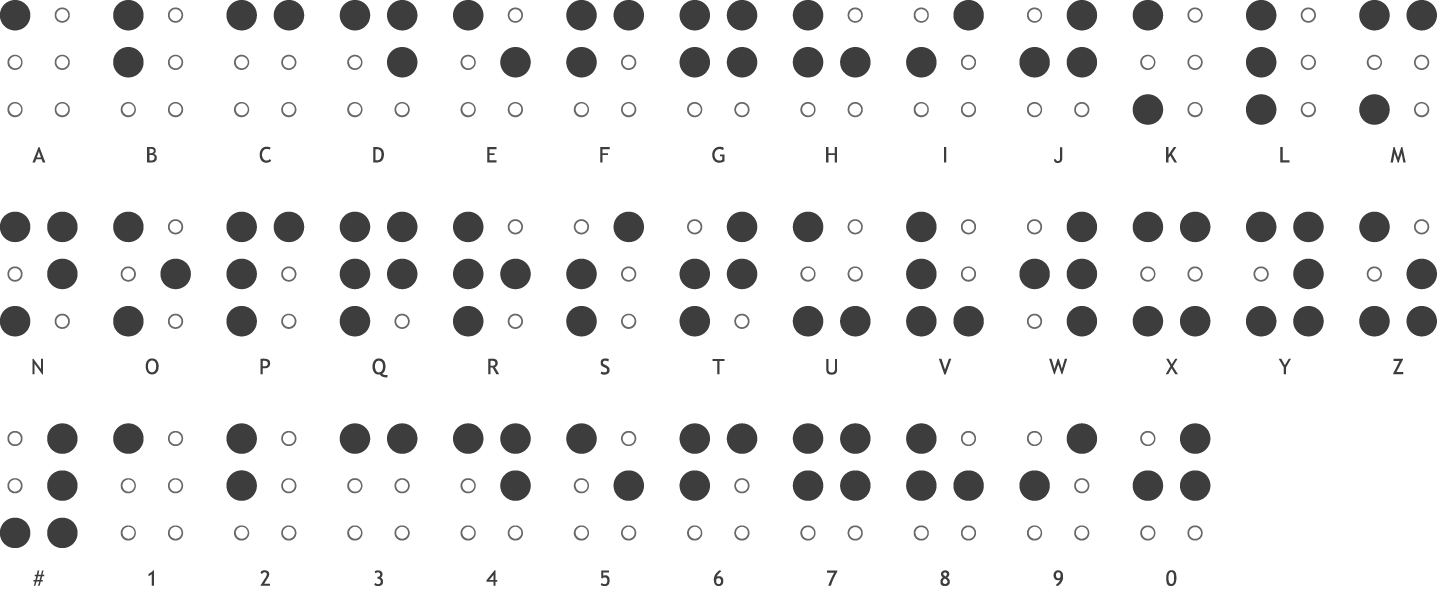
\includegraphics[scale=0.17]{./pics/braille}\cite{braille}
	 	\caption{Links sieht man einen Klappentelegraphen. Rechts das englische Braille-Alphabet. }
	  	\label{fig:braille}
	\end{figure}
\newpage
\section{Theoretische Grundlagen}

Im Folgenden werden Datenstrukturen, Operationen und Methoden eingeführt, die wir in dieser Arbeit benötigen werden.

\subsection{Operationen auf Strings}

Sei das Alphabet $\Sigma$ definiert als eine Menge von Zeichen, dann bezeichnet $\Sigma^{*}$ die Menge aller Worte, die aus dem Alphabet gebildet werden können. Jedes dieser Worte bezeichnet man als String.
	Sei $s$ ein String mit der Länge $n$.
	
	\begin{definition}[Länge]
		Sei $|s|$ die Länge des String $s$, das heißt die Anzahl von Zeichen in $s$.
	\end{definition}
	
	\begin{definition}[Leerstring]
		Sei $\varepsilon \in \Sigma$* der leere String. Es gilt $|\varepsilon|$ = 0.
	\end{definition}
	
	\begin{definition}[Symbolzugriff]
		Für $x \in \mathbb{N}$ und $x \leq n$ sei $s[x]$ das $x$-te Zeichen aus $s$.
	\end{definition}
	
	\begin{definition}[Teilstring]
		Für $x,y \in \mathbb{N}$ und $1 \leq x < y \leq n$ sei $s[x,y]$ die Zeichenfolge vom $x$-ten bis zum $y$-ten Zeichen aus $s$, $s$[x] und $s$[y] einschließlich.
	\end{definition}
	
	\begin{definition}[Suffix]
		 Für $x \in \mathbb{N}$ und $x \leq n$ sei $s[x..]$ das $x$-te Suffix von $s$. Also gilt $s[x..] = s[x,n]$.
	\end{definition}
	
\subsection{Suffix-Tree}

\begin{definition}[Suffix-Tree]
		Ein Suffix-Tree eines Strings $s$ ist ein Baum mit $n$ Blättern. Alle inneren Knoten erfüllen folgende Bedingungen:
		\begin{itemize}
			\item Jeder Knoten hat mindestens 2 Kinder.
			\item Jede Kante ist mit einem nicht-leeren Teilstring von $s$ markiert.
			\item Die Markierung ausgehender Kanten eines Knotens beginnen nicht mit dem gleichen Zeichen.
			\item Die Konkatenation von allen Zeichen auf dem Pfad von der Wurzel zum Blatt $i$ ist das $i$-te Suffix $s[i..]$ von $s$.
		\end{itemize}
		\begin{beispiel}[Suffix-Tree]
			$s$ = \texttt{ananas\$}
			\begin{figure}[h]
				\centering
				  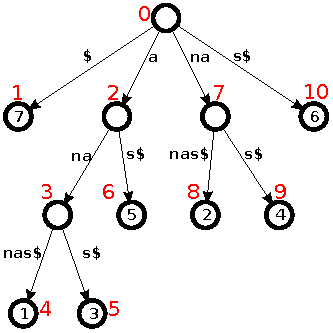
\includegraphics[scale=0.8]{./pics/ananas_suffixTree_inorder}
				  \cite{suffixtreeurl}
				  \caption{Diese Abbildung zeigt den Suffix-Tree zu $s$ = \texttt{ananas\$}. Die Blätter sind hierbei nummeriert. Der String auf dem Pfad von der Wurzel zum Blatt $i$ repräsentiert das Suffix $s[i..]$. Die roten Zahlen an den Knoten sind durch eine Pre-Order-Nummerierung entstanden. Im Folgenden nennen wir diese roten Zahlen IDs, da wir einen Knoten an seiner ID eindeutig identifizieren können. }
				  \label{fig:suffixTree}
			\end{figure}
		\end{beispiel}
		
	\end{definition}
	


	
\section{Idee der LZ78 Variante}

Um die Grundidee des Verfahrens, das wir in dieser Arbeit entwickeln, zu erläutern, betrachten wir im Folgenden zunächst LZ78.

\subsection{LZ78}\label{lz78_sec}

LZ78 wurde 1978 von Jacob Ziv und Abraham Lempel erfunden\cite{lempelziv78} und ist ein Verfahren zur Textkompression. Es benutzt dabei ein \textit{adaptives Wörterbuch}, das heißt für jeden Eingabetext wird ein anderes Wörterbuch erzeugt. LZ78 unterteilt den Eingabetext in Faktoren. Dabei ist jeder Faktor der längste, gleiche Substring im bisher gelesenen Eingabetext (ausschließlich des gerade zu berechnenden Faktors) plus das nächste Zeichen. Ein Faktor wird dabei als Tupel $(x,c)$ dargestellt, wobei $x$ der Index des Prefix ist und $c$ das zusätzliche Zeichen. Eine Einschränkung, wie weit der referenzierte Teilstring zurückliegen darf, gibt es hierbei nicht. Wenn $p$ Faktoren erstellt wurden, lässt sich der Index mit $\lceil\log p\rceil$ Bits darstellen. In der Praxis kann dieses Wörterbuch nicht unendlich groß werden. Daher löscht man dieses Wörterbuch, falls kein Speicher mehr verfügbar ist, und arbeitet mit einem leeren Wörterbuch und dem restlichen Eingabetext weiter.\\
Eine abstrakte Datenstruktur, um die Faktoren darzustellen, ist ein Trie bzw. hier der sog. LZ78-Trie. Jeder Knoten des LZ78-Tries enthält den Index des Faktors, den er repräsentiert. Hierbei ist der String auf dem Pfad von der Wurzel bis zum Knoten gleich dem Teilstring des Eingabetextes, der durch den Faktor dargestellt wird. \cite[S.225]{bellTextCompression}\\
Dieses Verfahren wird in Abbildung \ref{fig:lz78} nun am Beispiel von $T = \texttt{ananas\$}$ verdeutlicht:

 	
	\begin{figure}[h]
	\begin{tabular}[t]{cc}
		\begin{tabular}[b]{l c c c c c}\hline
			& 1 & 2 & 3 & 4 & 5 \\ \hline
		   Textteil & \texttt{a} & \texttt{n} & \texttt{an} & \texttt{as} & \texttt{\$}\\ \hline
		   Faktorzerlegung & (-,\texttt{a}) & (-,\texttt{n}) & (1,\texttt{n}) & (1,\texttt{s}) &  (-,\texttt{\$})\\ \hline
		\end{tabular} & 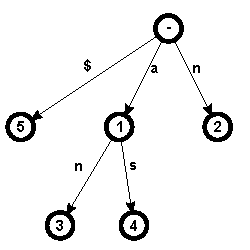
\includegraphics{./pics/ananas_LZ78Tree}
	\end{tabular}
	\caption{Links sieht man die Faktorisierung nach LZ78 und rechts den entsprechenden LZ78-Tree. Der $i$-te Faktor $(x,s)$ wird zu einem neuen Knoten $i$ mit $x$ als Elternknoten und die Kante $(x,i)$ wird mit $s$ beschriftet. Die Wurzel des Baumes beschriften wir mit '-', da sie keinen Faktor darstellt. Ein Faktor (-,s) ist somit ein Kindknoten der Wurzel.}
	\label{fig:lz78}
	\end{figure}

Den LZ78-Trie können wir zum Beispiel mithilfe \cite[Kapitel 6.3]{cics}	implementieren. Damit lässt sich der LZ78-Trie in $O(n)$ Zeit konstruieren und benötigt $2z + z \log \sigma$ Bits.\\
Die Berechnung einer LZ78 Faktorisierung benötigt jedoch viele Hilfsdatenstrukturen, zum Beispiel müssen wir speichern, bis zu welchem Buchstaben einer Kante die Faktorisierung fortgeschritten ist. An dieser Stelle zeigt sich der Vorteil der LZ78 Variante. Diese können wir einfacher berechnen, da wir zum Beispiel die Informationen über den Kantenfortschritt nicht speichern müssen. 
	

\subsection{LZ78 Variante}\label{LZ78 Variante}

In dieser Arbeit wollen wir eine Variante (im Folgenden LZ78V genannt) zu LZ78 aus Kapitel \ref{lz78_sec} entwickeln. LZ78V unterteilt den Eingabetext auch in Faktoren. Jedoch kann ein Faktor mehr als nur das nächste Zeichen an den referenzierten Teilstring anhängen. Die Information, welche Zeichen dies sind, bezieht LZ78V aus dem Suffix-Tree. Bei unserem Beispieltext $T = \texttt{ananas\$}$ folgt nach einen \texttt{'n'} immer ein \texttt{'a'}. Dies spiegelt sich im Suffix-Tree aus \autoref{fig:suffixTree} durch die Kante (0,7), die mit \texttt{'na'} beschriftet ist, wider. Mit LZ78V können wir nun beim ersten Lesen von \texttt{'n'} den Faktor (0, \texttt{'na'}) erstellen.
 Es ergibt sich die Faktorisierung aus \autoref{fig:lz78v}. \\
	\begin{figure}[h]
	\begin{tabular}[t]{c c c}
		\begin{tabular}[b]{l c c c}\hline
			& 1 & 2 & 3  \\ \hline
  		Textteil & \texttt{a} & \texttt{na} & \texttt{nas\$} \\ \hline
  		Faktorzerlegung & (-,\texttt{a}) & (-,\texttt{na}) & (2,\texttt{s\$}) \\ \hline
		\end{tabular} & \hspace{2cm} & 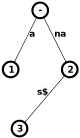
\includegraphics{./pics/ananas_LZ78VTree}\\\\
	\end{tabular}
	\caption{Links sieht man die Faktorisierung nach LZ78V und rechts den entsprechenden LZ78V-Tree. Der $i$-te Faktor $(x,s)$ wird zu einem neuen Knoten $i$ mit $x$ als Elternknoten und die Kante $(x,i)$ wird mit $s$ beschriftet. Im Gegensatz zum LZ78-Tree kann $s$ aber mehr als ein Zeichen beinhalten.}
	\label{fig:lz78v}
	\end{figure}
	
	Den LZ78V-Tree können wir mit zwei Arrays $A_1$ und $A_2$ repräsentieren. $A_1$ speichert hierbei Referenzen auf vorherige Faktoren bzw. '-' für keine Referenz. $A_2$ speichert die Strings, die ein Faktor an den referenzierten Faktor anhängt. So wäre $A_1[i] = x$ und $A_2[i] = s$ der $i$-te Faktor $(x,s)$ in der Array-Darstellung, mit $x \in \{1..z\} \cup \{-\}$ und $ s \in \Sigma^+$, wenn $z$ die Anzahl der Faktoren ist. Im Beispiel $T$ = \texttt{ananas\$} ergibt sich:\\\\
	\begin{tabular}{l c c c}
						\hline
							& 1 & 2 & 3 \\\hline
						$A_1$ & - & - & 2 \\\hline
						$A_2$	& \texttt{a} & \texttt{na} & \texttt{s\$}\\\hline
						
			
	\end{tabular}\\
	
	
LZ78V baut also wie LZ78 einen Tree auf. Vergleichen wir beide Trees aus unserem Beispiel, fällt auf, dass der LZ78V-Tree zwei Knoten weniger hat. Das heißt wir müssen weniger Informationen abgespeichert. Eine Kodierung des LZ78V-Trees entwickeln wir in einem späteren Abschnitt.\\
Gehen wir jedoch strikt nach dem oben beschriebenen Verfahren vor, so kann es auch zu einer schlechteren Faktorisierung als bei LZ78 kommen. Schlecht definieren wir hier über die Gesamtanzahl der Zeichen in der Faktorisierung. Je mehr Zeichen in $A_2$, desto schlechter ist die Faktorisierung. Betrachten wir beispielsweise den Text $T = \texttt{kananas\$}$. Lesen wir nun das \texttt{'k'} erstellt LZ78V direkt den Faktor $(-, \texttt{kananas\$})$ mit 8 Zeichen. Dies entsteht dadurch, dass sobald wir ein \texttt{'k'} lesen, LZ78V den kompletten String der Kante (0,7) des Suffix-Trees aus \autoref{fig:kananas} zu einem Faktor hinzufügt. Da \texttt{'k'} ein einzigartiges Zeichen in $T$ ist, enthält der Faktor des gesamten Text $T$. Eine Lösung zum Beispiel ist, $(x,s)$ nur in die Faktorisierung aufzunehmen, wenn der entsprechende Knoten im Suffix-Tree kein Blatt ist. Ansonsten nehmen wir nur das erste Zeichen von $s$.\\ Am Beispiel von $T = \texttt{kananas\$}$ ergibt sich somit folgeneder LZ78V-Tree in der Array-Darstellung:\\

\begin{tabular}{l c c c c c}
						\hline
							& 1 & 2 & 3 & 4 & 5\\\hline
						$A[1]$ & - & - & - & 3 & -\\\hline
						$A[2]$	& \texttt{k} & \texttt{a} & \texttt{na} & \texttt{s} & \texttt{\$}\\\hline
						
			
\end{tabular}\\




\begin{figure}[h]
	    \centering
		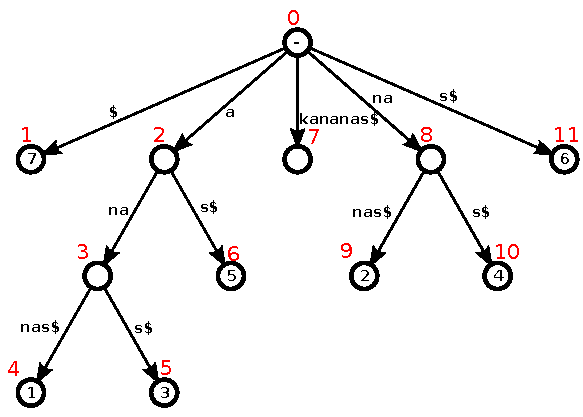
\includegraphics[scale=0.75]{./pics/kananas_suffixTree_inorder}
		 \caption{Diese Abbildung zeigt den Suffix-Tree zu $s$ = \texttt{kananas\$}. Die Blätter sind hierbei nummeriert. Der String auf dem Pfad von der Wurzel zum Blatt $i$ repräsentiert das Suffix $s[i..]$. Die roten Zahlen an den Knoten sind durch eine Pre-Order-Nummerierung entstanden und sind die IDs der Knoten.}
		 \label{fig:kananas}
\end{figure}

Diese Faktorisierung hat insgesamt 6 Zeichen, ist also besser als die Faktorisierung nach dem strikten Verfahren.

\section{Faktorisierung mit LZ78V}\label{factorisation}

In diesem Kapitel entwickeln wir einen Algorithmus und die dazu notwendigen Datenstrukturen, basierend auf der Grundidee aus Abschnitt \ref{LZ78 Variante}. 
Desweiteren definieren wir in \autoref{encode} einen \textit{Kodierer}, der die Faktorisierung kodiert und wir sie so effizient abspeichern können.
Abschließend stellen wir einen \textit{Dekodierer} vor, der aus einer Kodierung wieder die ursprüngliche Faktorisierung herstellt.

\subsection{SDSL-lite}
SDSL-lite ist eine C++11 Bibliothek, die speichereffiziente Datenstrukturen zur Verfügung stellt. Die benutzten Datenstrukturen dieser Bibliothek werden im Nachfolgenden an den passenden Stellen eingeführt\cite{sdsl}.

\begin{algorithm}
	\SetAlgoLined
	\SetAlgoNoEnd%
	\KwData{Eingabetext $T$ der Länge $n$}
	\KwResult{Vektor mit IDs(Repräsentation der Faktoren) und Vektor mit benutzzen Knoten}
	
	konstruiere Suffix-Tree aus $T$\;
	erstelle Bit-Vektor $used$ und Int-Vektor $factors$\;
	$pos \leftarrow 1$	\tcp*{aktuelle Textposition in $T$}
	\While{$pos \leq n$} {
		suche anhand $T[pos]$ den nächsten Knoten im Suffix-Tree\;\label{line:child}
		\If{aktueller Knoten in $used$ als benutzt markiert}{ \label{line:used}
			$pos \leftarrow pos + c_e(aktueller Knoten)$\;
			\tcc{$c_e$(Knoten) ist Anzahl Zeichen an der Kante zum Knoten}
			\textbf{continue}\;
		}
		\If{aktueller Knoten ist ein Blatt}{ \label{line:onlyFirstSym}
			$pos \leftarrow pos + 1$\;
		} \Else {
			setze Textposition entsprechend der Zeichen an der Kante weiter\; \label{line:textpos}
		}
		$pos \leftarrow pos + c_e(aktueller Knoten)$\;
		markiere aktuellen Knoten in $used$ als benutzt\;
	}
	
	\caption{LZ78V Faktorisierung mit Vektoren}
	\label{algo:factVec}
\end{algorithm}

\newpage

\subsection{Suffix-Tree Konstruktion}

Um aus dem Eingabetext einen Suffix-Tree zu konstruieren verwenden wir die Bibliothek SDSL-lite. Hiermit können wir einen sog. \textit{Compressed Suffix Tree} (CST) erzeugen. Dieser hat zur Laufzeit einen Speicherbedarf von 3$n$ + o($n$) + $\arrowvert$CSA$\arrowvert$ + $\arrowvert$LCP$\arrowvert$ Bits.\cite{sdsl} Jeder Knoten besitzt eine ID $i$, die wir durch eine Anfrage an den Baum in konstanter Zeit erhalten.
Sei $x$ die Anzahl von Knoten im Suffix-Tree, dann ist $i \in [0..x]$.


\subsection{Vektoren zur Faktorisierung}

Der Algorithmus benutzt zwei Vektoren. Diese erstellen wir wieder mithilfe von SDSL-lite.

\subsubsection{Bit-Vektor used}

Der Bit-Vektor $used$ besteht aus $x$ Bits, die mit 0 initialisiert werden. Dieser Vektor gibt an, ob ein Knoten mit der ID $i$ schon als Faktor benutzt wird.
Ist dies der Fall, so ist $used[i]=1$. Dieser Vektor benötigt $64*\lceil\dfrac{x}{64}+1\rceil$ Bits.\cite{sdsl}

\subsubsection{Int-Vektor factors}

Der Int-Vektor $factors$ ist zu Beginn leer. Wir füllen ihn im Laufe der Faktorisierung mit IDs von Knoten aus dem Suffix-Tree.  

\subsection{Abbruchbedingung der Faktorisierung}

Der Algorithmus bricht ab, wenn wir das Ende des Eingabetextes erreicht haben. Dies ist der Zeitpunkt, an dem die Faktorisierung abgeschlossen ist.

\subsection{Faktoren erstellen}

Der Startknoten jedes neuen Suchdurchlaufs ist die Wurzel des Suffix-Trees.
In Zeile \ref{line:child} des Algorithmus \ref{algo:factVec}  suchen wir anhand des aktuellen Zeichens aus dem Text den nächsten Knoten $k$ im Suffix-Tree. Diese Methode wird von SDSL-lite bereitgestellt und benötigt $O((t_{SA}+t_{SA^{-1}}) * \log \sigma + t_{LCP})$ Zeit. Hierzu sehen wir in einem späteren Abschnitt noch eine schnellere Alternative. In Zeile \ref{line:used} testen wir, ob $k$ schon als Faktor benutzt wird. Das bedeutet, wir haben den String  auf dem Pfad bis $k$ bereits durch einen Faktor dargestellt und können diesen nun referenzieren. Falls dies der Fall ist, setzen wir die Textposition um so viele Zeichen weiter, wie an der Kante zu $k$ stehen und suchen nach dem nächsten Knoten. Sobald wir einen Knoten $k$ gefunden haben, der noch nicht als Faktor benutzt wird, also für den $used[k]$ = 0 gilt, testen wir in Zeile \ref{line:onlyFirstSym}, ob der aktuelle Knoten ein Blatt ist. Falls ja, erhöhen wir die Textposition nur um 1, da nur das erste Zeichen der Kante zu $k$ zum Faktor hinzugefügt wird. Ist $k$ kein Blatt, setzen wir die Textposition um so viele Zeichen weiter, wie an der Kante zu $k$ stehen. Außerdem fügen wir die ID von $k$ an $factors$ an und markieren $k$ in $used$ als benutzt.

\subsection{Beispiel}\label{example:fact}

In diesem Abschnitt betrachten wir die Faktorisierung an unserem Beispieltext $T$ = \texttt{ananas\$}.\\
Der Suffix-Tree von $T$ aus \autoref{fig:suffixTree} hat 11 Knoten. Also ergibt sich nach der Initialisierung der Vektoren:
\begin{itemize}
	\item $used$ = [0,0,0,0,0,0,0,0,0,0,0]
	\item $factors$ = []
\end{itemize}

Nun beginnen wir den Text zu lesen. Das erste Zeichen ist ein \texttt{'a'}. Benutzen wir ausgehend von der Wurzel im Suffix-Tree die entsprechende Kante, gelangen wir zum Knoten mit der ID 2. Dieser Knoten ist noch nicht benutzt, da $used[2] = 0$. Somit fügen wir 2 an $factors$ an, setzen $used[2]$ = 1 und erhöhen die Textposition um 1. Es ergibt sich:
\begin{itemize}
	\item $used$ = [0,0,1,0,0,0,0,0,0,0,0]
	\item $factors$ = [2]
\end{itemize}

Nächstes Zeichen: \texttt{'n'}\\
Gehen wir von der Wurzel des Suffix-Trees die entsprechende Kante, gelangen wir zum Knoten mit der ID 7, der auch noch nicht benutzt ist. Die Textposition erhöhen wir um 2, da an der Kante zwei Zeichen stehen.

\begin{itemize}
	\item $used$ = [0,0,1,0,0,0,0,1,0,0,0]
	\item $factors$ = [2,7]
\end{itemize}

Nächstes Zeichen: \texttt{'n'}\\
Nun gelangen wir durch benutzen der entsprechenden Kante des Suffix-Trees von der Wurzel  wieder zum Knoten mit der ID 7. Diesen haben wir im letzen Durchlauf als benutzt markiert. Das heißt wir erhöhen die Textposition um 2 und suchen anhand des nächsten Zeichens \texttt{'s'} den nächsten Knoten im Suffix-Tree. Das ist der Knoten mit der ID 9. Allerdings ist dieser Knoten ein Blatt, das heißt wir erhöhen die Textposition nur um 1. Wir fügen die ID 9 an $factors$ an und markieren den Knoten als benutzt.

\begin{itemize}
	\item $used$ = [0,0,1,0,0,0,0,1,0,1,0]
	\item $factors$ = [2,7,9]
\end{itemize}

Nächstes Zeichen: \texttt{'\$'}
Wir gelangen zum Knoten mit der ID 1. Dieser ist noch nicht benutzt, also fügen wir die ID 1 an $factors$ an und markieren ihn als benutzt. Die Textposition erhöhen wir um 1, da der Knoten ein Blatt ist.

\begin{itemize}
	\item $used$ = [0,1,1,0,0,0,0,1,0,1,0]
	\item $factors$ = [2,7,9,1]
\end{itemize}

Das Ende des Textes ist erreicht. Somit ist die Abbruchbedingung erfüllt und die Faktorisierung abgeschlossen.

\hspace{20px}

Haben wir mit Algorithmus \ref{algo:factVec} die Vektoren $factors$ und $used$ gefüllt, verfügen wir über alle Informationen der Faktorisierung, die wir benötigen. Nun können wir mithilfe von Algorithmus \ref{algo:lz78v-tree} aus den beiden Vektoren konkrete Faktoren mit Referenz und anzuhängenden Symbolen entwickeln. Denn würden wir nur die Vektoren abspeichern, wäre es unmöglich daraus wieder den ursprünglichen Text zu rekonstruieren. Um die Faktoren zu speichern benutzen wir die Array-Darstellung aus Kapitel \ref{LZ78 Variante}.

\begin{algorithm}\label{algo:lz78v-tree}
	\SetAlgoLined
	\SetAlgoNoEnd%
	\KwData{Suffix-Tree, Bit-Vektor $used$, Int-Vektor $factors$}
	\KwResult{Arraydarstellung des LZ78V-Tree}
	erstelle Int-Vektor $N$\;
	erstelle \textit{rank}-Struktur auf $used$\;
	\For{$i\leftarrow$0 \KwTo $z-1$} {
		N[$used$.rank($factors[i]$)] = $i + 1$\;
	} \label{line:nFilled}
	erstelle $A_1$ und $A_2$\;
	\For{$j\leftarrow$0 \KwTo $x-1$} {
		\If{$used$[j]!=0} { \tcc{$used[j] = 0 \Leftrightarrow$ Knoten mit ID $j$ ist unbenutzt}
			$p\leftarrow$ Elternknoten im Suffix-Tree des Knotens mit der ID $j$\;
			\If{$p$ ist Wurzel des Suffix-Trees} {
				$A_1[N[used.rank(j)]] \leftarrow 0$\;
			} \Else {
				$A_1[N[used.rank(j)]] \leftarrow N[U.rank(p.id())]$\;
				\tcc {id() gibt die ID eines Knotens zurück}
			}
			\If{Knoten mit ID j im Suffix-Tree ist ein Blatt} {
				$A_2[N[used.rank(j)]] \leftarrow$ erstes Zeichen der Kante zum Knoten mit ID j\;
			} \Else {
				$A_2[N[used.rank(j)]] \leftarrow$ ganzer String der Kante zum Knoten mit ID j\;
			}		
		}
	}
	
	\caption{LZ78V-Tree}
	\label{algo:lz78v-tree}
\end{algorithm}


\subsection{rank-Struktur auf used}

Eine \textit{rank}-Struktur auf einem Bit-Vektor $v$ ist eine Funktion $rank_v$ : $[1..|v|] \rightarrow \mathbb{N}_0$ die jedem Index $i$ die Häufigkeit von 1-Bits im Vektor bis zum Index $i$ zuordnet\cite[S. 39]{munroTables}.


\subsection{Int-Vektor N}

Der Int-Vektor $N$ hat $z$ Einträge. Dieser Vektor speichert für jede ID aus $factors$, eine Faktor-ID, die angibt den wievielten Faktor der entsprechende Knoten repräsentiert. Um diesen Vektor zu füllen, gehen wir $factors$ einmal von links nach rechts durch. Wir setzen dabei $N[used.rank(factors[j])] = j$ für jeden Eintrag in $factors$ an der Position $j$.
 


\subsection{Füllen von $A_1$ und $A_2$}

$A_1$ füllen wir mit Referenzen auf Faktoren, $A_2$ mit Strings, die an den referenzierten Faktor angehangen werden. Beide Arrays haben die Länge $z$.
Nun können wir mithilfe von $used$, $N$ und dem Suffix-Tree die Arrays $A_1$ und $A_2$ füllen. Dazu durchlaufen wir $used$ einmal von links nach rechts durch und verfahren mit jedem Eintrag an Position $j$, der als nicht benutzt markiert ist, wie folgt:\\
Falls der Elternknoten von Knoten $j$  die Wurzel des Suffix-Trees ist, setze \\$A_1[N[used.rank(j)]] = 0$. Ansonsten setze $A_1[N[used.rank(j)]] = N[U.rank(p.id())]$.
$N[used.rank(j)]$ ist dabei die Faktor-ID des entsprechenden Knoten mit der Knoten-ID $j$. 
Auf diese Weise werden die Referenzen in $A_1$ richtig befüllt. Wollen wir $A_2$ füllen, müssen wir testen ob der Knoten mit der ID j im Suffix-Tree ein Blatt ist. Falls ja, speichern wir an der Position $N[U.rank(j)]$ in $A_2$ nur das erste Zeichen der Kante zum Knoten $j$. Andernfalls den gesamten String an der Kante. Dies löst das Problem von einzigartigen Zeichen im Eingabetext.

\begin{beweis}
	Sei $T$ = $s_1ks_2$ mit $s_1,s_2 \in \Sigma^+ \setminus \{k\}$ und $k \in \Sigma$. \\
	Sind wir beim Lesen von $T$ bei $k$ angelangt, landen wir im Suffix-Tree als nächstes immer zu einem Blatt über eine Kante, die mit $ks_2$ markiert ist.
	Die Faktorisierung wäre somit abgeschlossen, obwohl $s_2$ noch viel Potenzial auf eine gute Faktorisierung haben kann. Somit nehmen wir nur $k$ in die Faktorisierung auf und arbeiten mir $s_2$ weiter.
\end{beweis}

\subsubsection{Beispiel}

In diesem Abschnitt betrachten wir beispielhaft die Konstruktion des LZ78V-Tree. Als Eingabe benutzen wir die Ergebnisse aus dem Beispiel in Kapitel \ref{example:fact} und konstruieren mithilfe des Algorithmus \ref{algo:lz78v-tree} die Array-Darstellung des LZ78V-Tree.\\

\begin{itemize}
\item Eingabe: 
	\begin{itemize}
		\item Suffix-Tree aus Abbildung \ref{fig:suffixTree}
		\item Bit-Vektor $used$ aus dem Ergebnis von Kapitel \ref{example:fact}: \\
		$used$ = [0,1,1,0,0,0,0,1,0,1,0]
		\item Int-Vektor $factors$ aus dem Ergebnis von Kapitel \ref{example:fact}: \\
		$factors$ = [2,7,9,1]
	\end{itemize}
	
\item Nach Zeile \ref{line:nFilled}: $N = [3,0,1,2]$
\item Ergebnis:
	\begin{itemize}
		\item $A_1 = [0 ,0 , 2, 0]$
		\item $A_2 = [\texttt{a}, \texttt{na}, \texttt{s}, \texttt{\$}]$
	\end{itemize}
\end{itemize}

\section{Kodierung}\label{encode}

Wurde aus einem Eingabetext $T$ gemäß Algorithmus \ref{algo:factVec} eine Faktorisierung erzeugt und daraus gemäß Algorithmus \ref{algo:lz78v-tree} die Array-Darstellung des LZ78V-Trees, können wir mit der \textit{Kodierung} beginnen. Durch die Kodierung können wir die Array-Darstellung effizient speichern.\\
Zuerst konstruieren wir aus der Array-Darstellung einen String. Diesen String nennen wir Ergebnisstring $s$. Dazu hängen wir abwechselnd die Einträge aus $A_1$ und $A_2$ hintereinander, getrennt durch ein Zeichen, das in keinem Text vorkommen kann. Daher nehmen wir als Trennzeichen das ASCII Zeichen '$\setminus$x1B'. Dieses Trennzeichen wird im Folgenden als \texttt{'|'} dargestellt.
In unserem Beispiel $T$ = \texttt{ananas\$} erhalten wir so den Ergebnisstring \\$s$ = \texttt{0|a|0|na|2|s|0|\$|}.
Dieser Ergebnisstring $s$ soll nun kodiert werden. Hierzu wird der nachfolgende Kodierer eingeführt.

\subsection{Kanonische Huffman Kodierung}

Die kanonische Huffman Kodierung ordnet jedem Symbol einen präfixfreien Code zu. Präfixfrei bedeutet, dass es keinen Code gibt, der Präfix eines anderes Codes ist.
Diese Kodierung hat gegenüber der in der Literatur üblichen Huffman Kodierung\cite[S. 141ff]{dataCompressionHeld} den Vorteil, dass sie speichereffizienter ist und die Dekodierung schneller ist. \cite[S. 335]{managingGigabytes}

\begin{algorithm}[t]
	\SetAlgoLined
	\SetAlgoNoEnd%
	\KwData{Array $H$ der Länge $w$ mit Häufigkeiten aller $w$ Symbole}
	\KwResult{Code Längen der Symbole}
	/* Phase Eins */\\
	erstelle ein Array $A$ mit Länge $2n$\;
	\For{$i\leftarrow0$ \KwTo $w$ } {
		lese $h_i$\tcc*{$h_i$ ist Häufigkeit des $i$-ten Symbols}
		$A[w+i]\leftarrow h_i$\;
		$A[i]\leftarrow w + i$\;
	} 
	$h\leftarrow w$\;
	baue einen Min-Heap von $A[1..w]$\;
	/*Phase zwei*/\\
	\While{h > 1} {
		$m_1 \leftarrow A[1]$\;
		$A[1] \leftarrow A[h]$\;
		$h \leftarrow h - 1$\;
		
		stelle für $A[1..h]$ Heap-Eigenschaft wieder her\;
		$m_2 \leftarrow A[1]$
		
		$A[h+1] \leftarrow A[m_1] + A[m_2]$\;
		$A[1] \leftarrow h+1$\;
		$A[m_1] \leftarrow A[m_2] \leftarrow h + 1$\tcc*{speichere Elternverweise}
		stelle für $A[1..h]$ Heap-Eigenschaft wieder her\;	
	}
	/*Phase drei*/\\
	\For{$i\leftarrow w + 1$ \KwTo $2w$ } {
		$depth\leftarrow 0$\;
		$node\leftarrow i $\;
		\While{$node > 2$} {
			$depth\leftarrow depth + 1$\;
			$node\leftarrow A[r]$\;
		}
	}


	\caption{Berechne Code-Längen der Symbole \cite[S. 341]{managingGigabytes}}
	\label{algo:huf-codeLength}
\end{algorithm}

Algorithmus \ref{algo:huf-codeLength} ist der erste Teil der Berechnung der kanonischen Huffman Kodierung. Hier berechnen wir für jedes Symbol des Eingabetextes, wie lang der entsprechende Code für das Symbol ist. Dabei bauen wir uns mithilfe eines \textit{Min-Heaps} einen \textit{Huffman-Tree}, an dem wir die Code-Längen für alle Symbole ermitteln können.

\subsubsection{Huffman-Tree}

Um einen Huffman-Tree zu einer Menge von Symbolen zu konstruieren, erstellen wir für jedes Symbol einen Knoten und ordnen diesem die Häufigkeit des Symbols zu. Dann fügen wir immer die beiden Knoten mit der geringsten Häufigkeit zu einem neuen Teilbaum zusammen. Die Wurzel dieses Baums markieren wir mit der Summe der Häufigkeiten der beiden Kindknoten.
Dies wiederholen wir solange, bis nur noch ein Baum übrig ist. Dieser ist der \textit{Huffman-Tree} der Eingabemenge\cite[S. 39]{storerDataCompression}. Im Beispiel von $s$ = \texttt{0|a|0|na|2|s|0|\$|} sehen wir den Huffman-Tree in \autoref{fig:huffman_tree}.

	\begin{figure}[h]
		\begin{center}
		
		 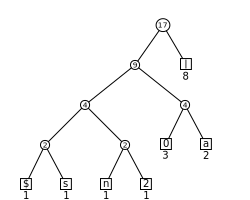
\includegraphics[scale=0.9]{./pics/huffman_Tree}
		 \end{center}
		
		\caption{Huffman-Tree zu $s$ = \texttt{0|a|0|na|2|s|0|\$|}. Die Blätter enthalten die Symbole. Darunter sehen wir die Häufigkeiten der Symbole. Die restlichen Knoten sind jeweils mit der Summe der Häufigkeiten in den entsprechenden Teilbäumen markiert.}
		\label{fig:huffman_tree}
	\end{figure}
	
Die Code-Längen der einzelnen Symbolen entsprechen dann der Tiefe im Huffman-Tree. So hat das Symbol '\$' die Code-Länge 4.


\subsubsection{Min-Heap}\label{min-heap}

Ein \textbf{(binärer) Heap} ist ein Binärbaum, dessen Knoten je ein Element einer Menge $X$ enthalten. Jeder Knoten erfüllt bezüglich einer totalen Ordnung $(X,\geq)$ die \textit{Heap-Eigenschaft}. Diese Eigenschaft ist wie folgt definiert:

\begin{definition} [Heap-Eigenschaft]
	\textbf{Gegeben:} Eine Menge $X$ und eine Relation $\geq$.\\
	Sei $x_{l}$ der linke und $x_{r}$ der rechte Kindknoten von $x$, so gilt:\\
	\begin{center}{$x_{l} \geq x$ und $x_{r} \geq x$}\end{center}
	 
\end{definition}

Ein \textit{Min-Heap} ist ein Heap, dessen Elemente die Relation $\geq$ erfüllen. Das heißt jeder Kindknoten enthält ein Element, das mindestens so groß ist wie das seines Elternknotens. Abbildung \ref{fig:min_heap_example} zeigt beispielhaft einen \textit{Min-Heap} $(\mathbb{N}, \geq )$.

\begin{figure}[h]
	    \centering
		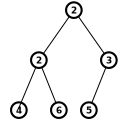
\includegraphics[scale=0.9]{./pics/min_heap_example}
		 \caption{Beispiel eines \textit{Min-Heaps} $(\mathbb{N}, \geq )$.}
		 \label{fig:min_heap_example}
\end{figure}

Eine effiziente Darstellung eines \textit{Heaps} ist ein Array $H$, was folgende Eigenschaften erfüllt:

\begin{itemize}
	\item Die erste Stelle von $H$ ist die Wurzel des Baums. \label{heap_array_prop_1}
	\item Der linke Kindknoten des $i-ten$ Knotens steht an der Stelle $2i$.
	\item Der rechte Kindknoten des $i-ten$ Knotens steht an der Stelle $2i + 1$.
	\item Der Vaterknoten des $i-ten$ Knotens steht an der Stelle $\lfloor\frac{i}{2}\rfloor$. ($i>1$)
\end{itemize}
	
In Abbildung \ref{fig:array_heap} sehen wir die Array-Darstellung des Baums aus Abbildung \ref{fig:min_heap_example}.

\begin{figure}[h]
	\centering
	
		\begin{tabular}[h]{|l|c|c|c|c|c|c|}\hline
			$i$ & 1 & 2 & 3 & 4 & 5 & 6\\ \hline
		   H[$i$] & 2 & 2 & 3 & 4 & 6 & 5\\ \hline
		   
		\end{tabular} 
		\caption{Array-Darstellung des Baums aus Abbildung \ref{fig:min_heap_example}.}
		\label{fig:array_heap}
\end{figure}

Ein Zugriff auf das kleinste Element des \textit{Min-Heaps} ist in $O(1)$ Zeit möglich, da das kleinste Element des Heaps immer an der ersten Stelle liegt.
Fügen wir ein neues Element in den Heap ein oder Löschen ein Element, so muss die \textit{Heap-Eigenschaft} weiterhin gelten. Da die Höhe eines Heaps logarithmisch von der Anzahl $n$ der Elemente im Heap abhängt und wir die Eigenschaft nach dem Löschen und Einfügen auf dem Pfad von der betroffenen Stelle bis zur Wurzel wiederherstellen müssen, benötigen Einfüge- und Löschoperationen $O(\log n)$ Zeit. \cite[S.115ff]{introductionToAlgorithms}
\vspace{40px}

Im Folgenden betrachten wir die drei Phasen von Algorithmus \ref{algo:huf-codeLength} und erläutern, wie wir mithilfe eines Min-Heaps einen Huffman-Tree konstruieren und an diesem die Code-Längen ermitteln. \\
In \textbf{Phase Eins} lesen wir in die zweite Hälfte $A[w+1..2w]$ alle Häufigkeiten der vorkommenden Sybole ein. Diese Häufigkeiten finden wir im Array $H$, wobei $H[i]$ die Häufigkeit des $i-ten$ Symbols angibt. Die Werte der ersten Hälfte $A[1..w]$ dienen als Zeiger auf eine Häufigkeit aus der zweiten Hälfte. $A$ können wir auch als eine Array-Darstellung eines Binärbaums verstehen. Betrachten wir im Beispiel den Ergebnisstring $s$ = \texttt{0|a|0|na|2|s|0|\$|}. Somit haben wir eine Symbolliste $Sym = [\texttt{0,|,a,n,2,s,\$}]$ und Häufigkeiten \\$H =[3,8,2,1,1,1,1] $, sodass $H[i]$ die Häufigkeit in $s$ von $Sym[i]$ angibt. Wir erhalten so:
\begin{center}
	$A = [8,9,10,11,12,13,14,3,8,2,1,1,1,1]$
\end{center}

Dann bauen wir in Zeile 9 aus der ersten Häfte einen Min-Heap. Wir vergleichen jedoch nicht die Elemente direkt, sondern die Werte auf die sie referenzieren. So definieren wir einen Min-Heap $(\mathbb{N}, \succeq)$ mit $\succeq(x,y) \mapsto A[x] \succeq A[y]$.

Min-Heap mit der ersten Häfte von $A$:

\begin{figure}
	\begin{center}
		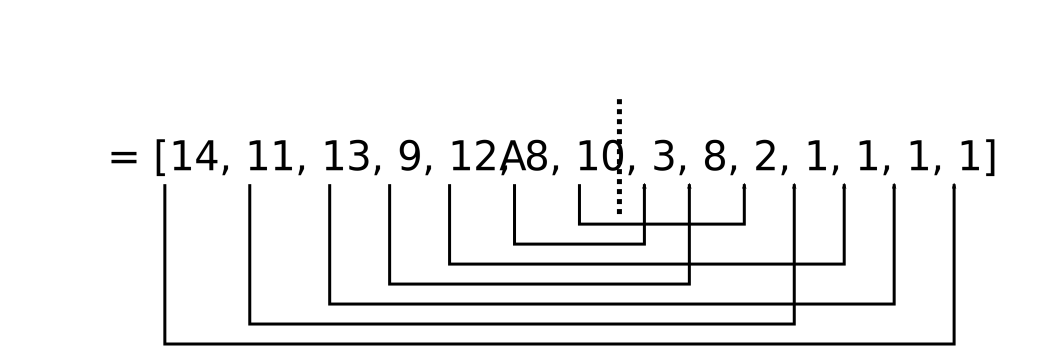
\includegraphics[scale=0.3]{./pics/A_heap}
		\caption{Hier sehen wir die Array-Darstellung des Min-Heaps aus dem Beispiel. Bis zu der gestrichelten Trennlinie gehören die Einträge zum Min-Heap. Die Pfeile verdeutlichen die Zeiger auf die Werte der zweiten Hälfte.}
		\label{A_heap}
	\end{center}
\end{figure}
\newpage
\autoref{fig:buildHeap} zeigt die Baumdarstellung des Min-Heaps. Die erste Hälfte von $A$ kann man dabei als IDs der Knoten verstehen, die zweite Hälfte als Werte innerhalb der Knoten.\cite[S. 342]{managingGigabytes}

\begin{figure}[h]
\centering
	  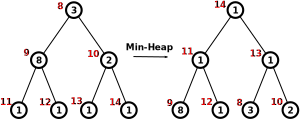
\includegraphics[scale=0.9]{./pics/build-Heap}
	  \caption{Diese Abbildung zeigt beispielhaft das Array $A$ in der Baumdarstellung vor und nachdem wir aus der ersten Häfte ein Min-Heap konstruiert haben. Die roten Zahlen sind aus der ersten Häfte, die schwarzen aus der zweiten Hälfte von $A$.}
	  \label{fig:buildHeap}
\end{figure}



In \textbf{Phase zwei} konstruieren wir aus $A$ einen Huffman-Tree. Dazu entfernen wir die Referenz auf den kleinsten Wert aus dem Heap und speichern ihn in $m_1$. Diese ist gemäß der Heap-Eigenschaft in A[1] zu finden. Außerdem überrschreiben wir $A[1]$ mit $A[h]$. Wir verringern $h$ um 1 und stellen die Heap-Eigenschaft im Bereich $A[1..h]$ wieder her. So hat sich die Größe des Heaps um 1 verringert. Nun speichern wir wieder die Referenz auf den kleinsten Wert aus dem Heap in $m_2$. In die freie Position $A[h+1]$ schreiben wir nun die Summe der beiden Häufigkeiten auf die $m_1$ und $m_2$ verweisen. An $A[m_1]$ und $A[m_2]$ schreiben wir $h+1$, also die Referenz auf den Elternknoten mit der Summe ihrer beiden Häufigkeiten. Nun stellen wir die Heap-Eigenschaft in $A[1..h]$ wieder her und beginnen von vorn. Dies wiederholen wir solange wie $h > 1$ gilt. 
Dieses Vorgehen verdeutlichen wir in \autoref{fig:A_heap_ilus}, indem wir im Beispiel die erste Iteration von Phase zwei illustrieren. 


\begin{figure}[h]
\centering
	  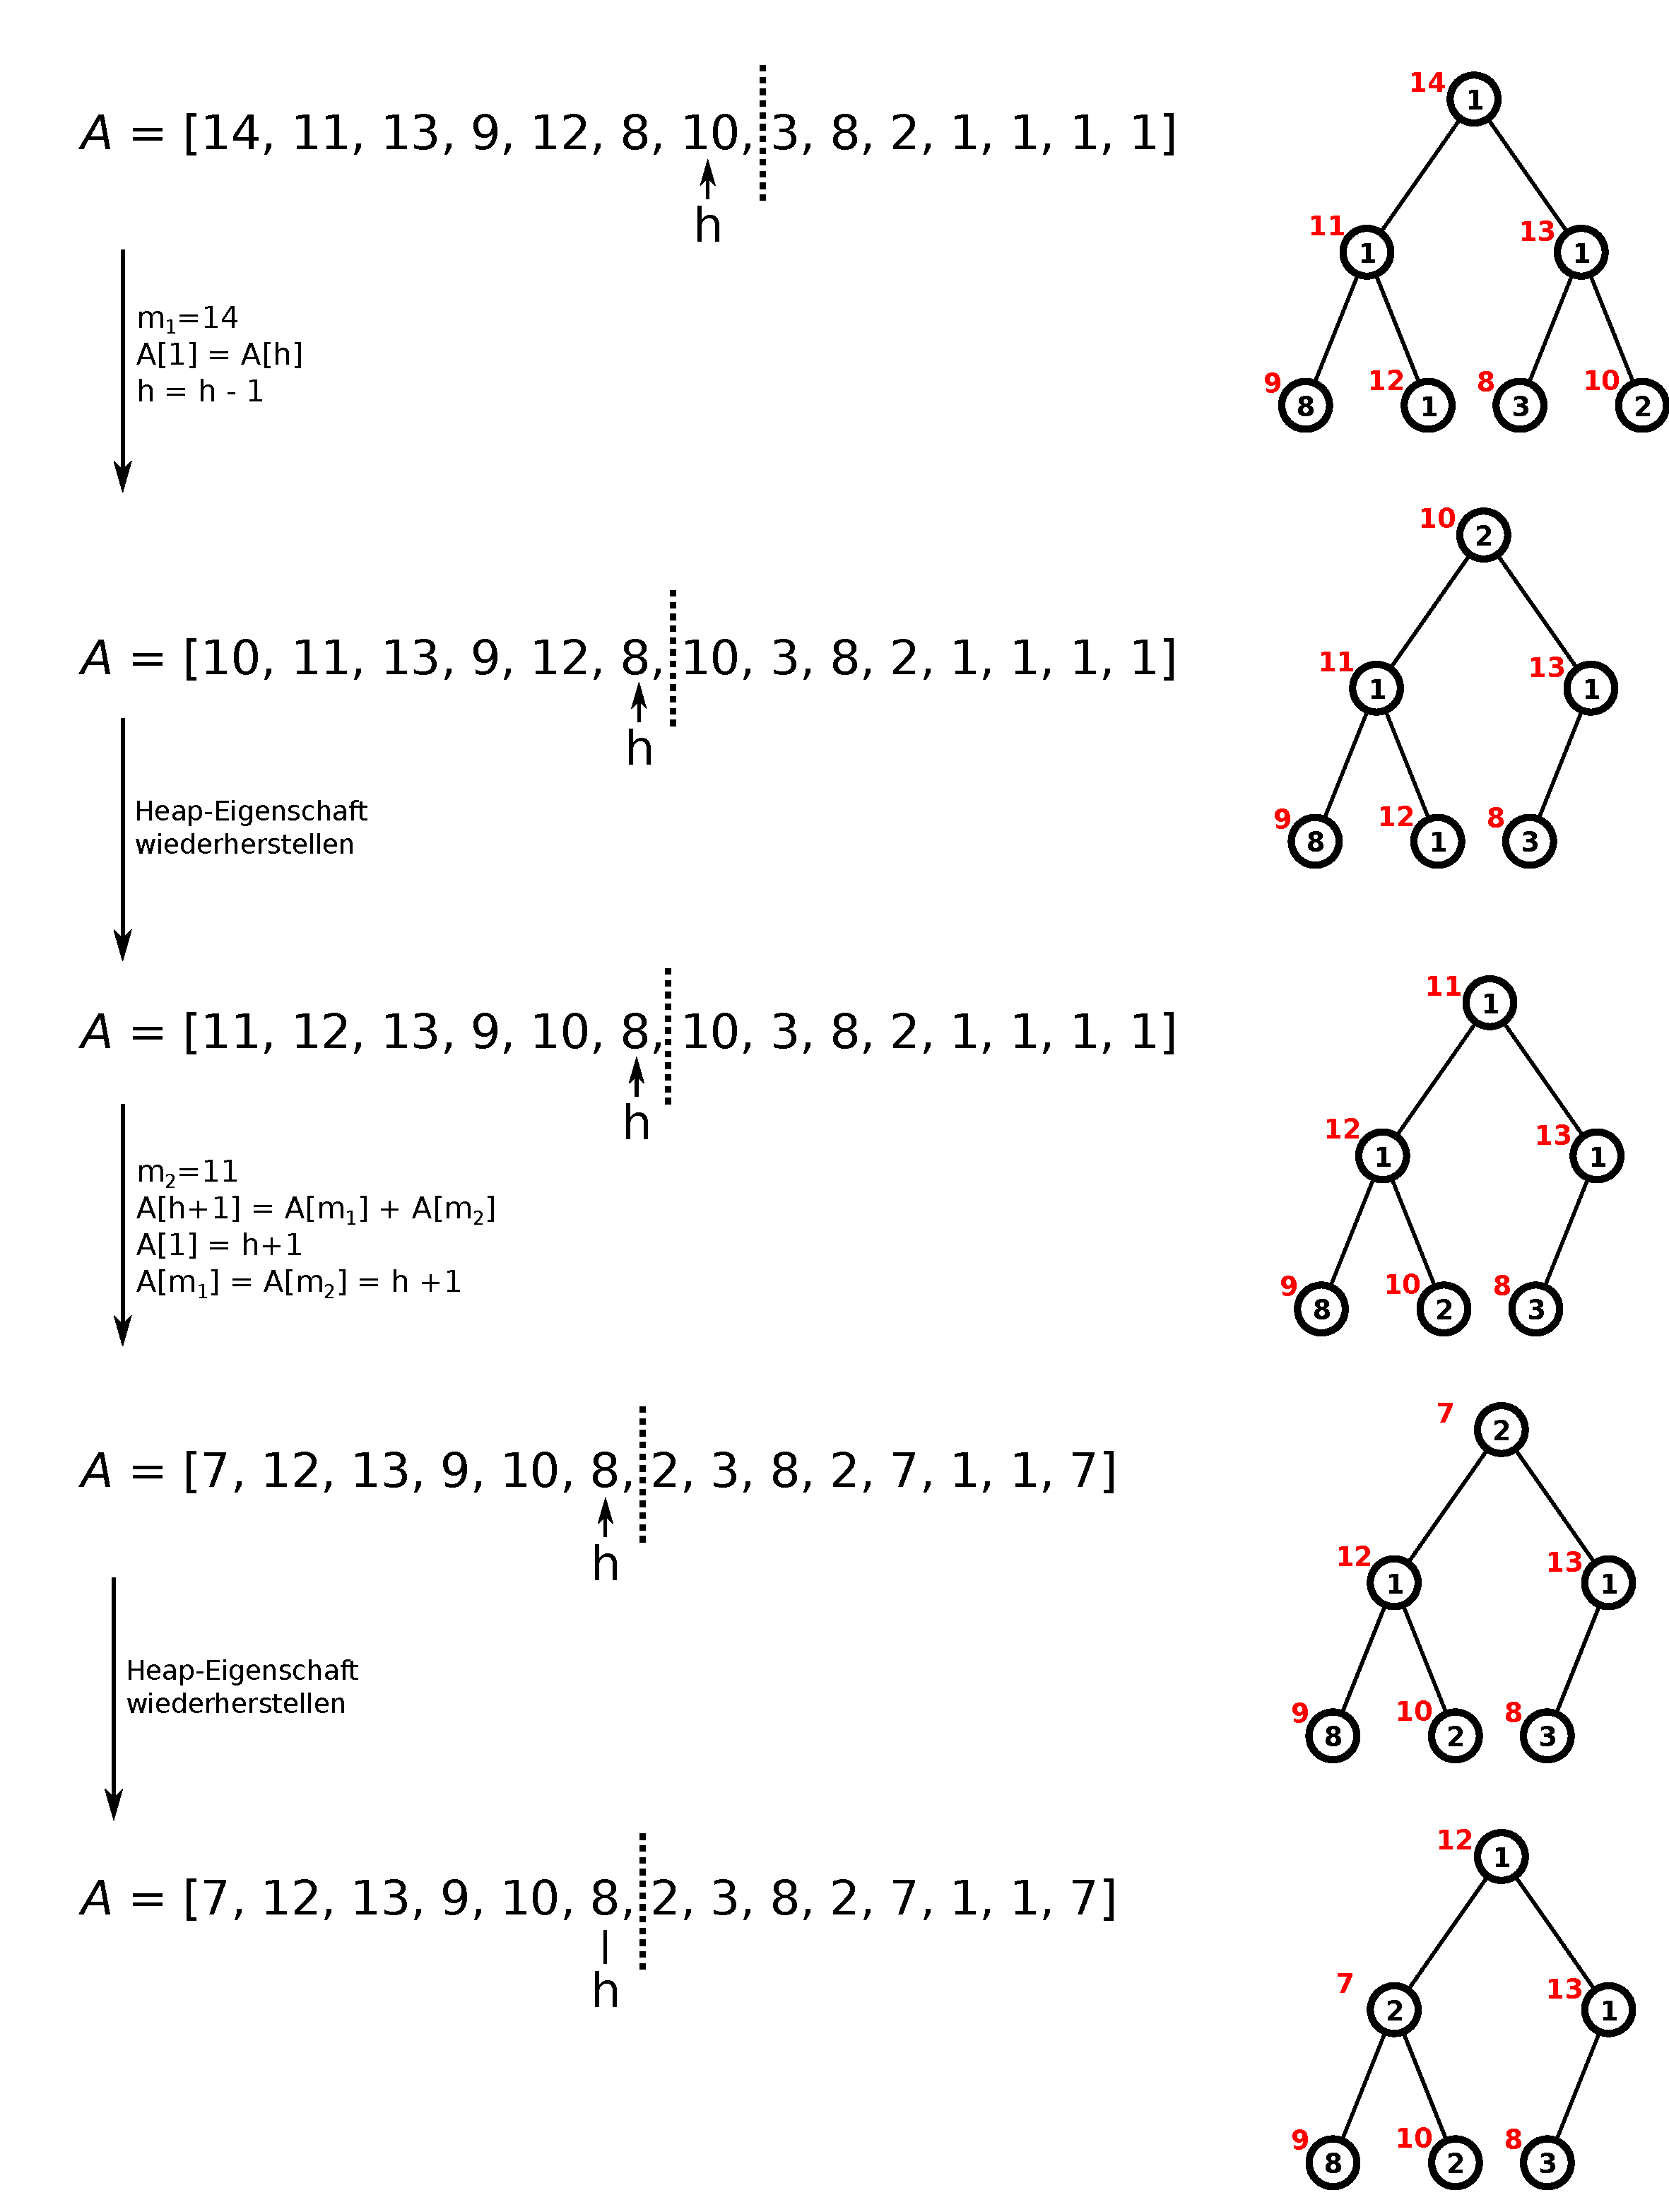
\includegraphics[scale=0.25]{./pics/A_heap_ilus}
	  \caption{Diese Abbildung zeigt die erste Iteration von Phase zwei des Algorithmus \ref{algo:huf-codeLength}. Links sehen wir die Array-Darstellung und rechts die Baumdarstellung der Heap-Struktur. An den Pfeilen sehen wir die Operationen, die in den Übergängen passieren. }
	  \label{fig:A_heap_ilus}
\end{figure}

Als Endergebnis von Phase zwei erhalten wir in unserem Beispiel:

\begin{center}
	$A[2,17,2,3,3,5,5,7,2,4,6,4,6,7]$
\end{center}

$A[1]$ enthält hierbei immer 2, da in $A[2]$ der einzige Knoten des Heaps gespeichert ist. Alle anderen Einträge in $A$ sind Verweise auf Elterknoten. \cite[S. 342ff]{managingGigabytes} Diese Verweise nutzen wir in Phase 3, um die Code-Längen zu ermitteln.



In \textbf{Phase 3} ermitteln wie die Code-Länge für jedes Symbol. Dazu beginnen wir an der Stelle $w + 1$ und verfolgen die Verweise auf den Elternknoten, bis wir an der Wurzel angelangt sind. Die ermittelte Länge speichern wir an der Stelle $w + 1$ ab. Dies wiederholen wir für jede Stelle aus $A[w+2..2w]$. Am Ende befindet sich die Code-Länge für Symbol $i$ in $A[w+i]$.\cite[S. 344]{managingGigabytes}


\begin{algorithm}
	\SetAlgoLined
	\SetAlgoNoEnd%
	\KwData{Array $L$ mit Code-Längen von $w$ Symbolen, $l_i$ ist Code-Länge von Symbol $i$}
	\KwResult{Array mit Integern für Codes}
	$max \leftarrow$ maximale Code-Länge\;
	\For{$m\leftarrow 1$ \KwTo $max$} {
		$num[m] \leftarrow 0$\;
	}
	\For{$i\leftarrow 1$ \KwTo $w$} {
		$num[l_i] \leftarrow num[l_i] + 1$\;
	}
	\tcp{$num[i]$ = Anzahl Codes der Länge i}
	$firstcode[max] \leftarrow 0$\;
	\For{$m\leftarrow max - 1$ \textbf{downto} 1} {
		$firstcode[m] \leftarrow (firstcode[m+1] + num[m+1])/2$\;
	}
	\For{$m \leftarrow 1$ \KwTo $max$} {
		$nextcode[m] \leftarrow firstcode[m]$
	}
	\For{$i \leftarrow 1$ \KwTo $n$} {
		$codeword[i] \leftarrow nextcode[i]$\;
		$nextcode[l_i] \leftarrow nextcode[l_i] + 1$\;
	}
	
	
	
	\caption{Symbolen einen kanonischen Huffman Code zuweisen \cite[S. 338]{managingGigabytes}}
	\label{algo:huf-assignCode}
\end{algorithm}

Haben wir die Code-Längen für jedes Symbol berechnet, können wir mithilfe von Algorithmus \ref{algo:huf-assignCode} für jedes Symbol einen Code in Dezimaldarstellung berechnen. Die rechten $l_i$ Bits dieser Dezimalzahl in Binärdarstellung sind der Code für das Symbol $i$.\\
Das Array $num$ speichert für jede Code-Länge bis $max$ wie oft sie in $L$ vorkommt. In $firstcode$ berechnen wir für jede Code-Länge den ersten Code. Dieser ist abhängig von $firstcode$ und $num$ des um 1 längeren Codes. Das Ergebnis dieses Algorithmus ist in $cordword$ gespeichert. Für unser Beispiel sieht das Ergebnis so aus:
\newpage
\begin{table}
		\begin{center}
		
		\begin{tabular}[h]{|c|c|c|l|}\hline
			Symbol & Code-Länge $l_i$  & $codeword[i]$ & Code\\ \hline
 		 	\texttt{0} & 3 & 3 & 011		\\ \hline
 			\texttt{|} & 1 & 1 & 1		\\ \hline
			\texttt{a} & 3 & 2 & 010		\\ \hline
 			\texttt{n} & 4 & 1 & 0001	\\ \hline
 			\texttt{2} & 4 & 3 & 0011	\\ \hline
  			\texttt{s} & 4 & 0 & 0000	\\ \hline
  			\texttt{\$} & 4 & 2 & 0010	\\ \hline
		\end{tabular} 
		\end{center}
		\caption{Diese Tabelle zeigt beispielhaft $codeword$ zum Ergebnisstring $s$ = \texttt{0|a|0|na|2|s|0|\$|}. Die Werte in $codeword$ sind Codes in Dezimaldarstellung. Der Code von Symbol $i$ ergibt sich aus den $l_i$ rechten Bits von $codeword[i]$ }
\end{table}


Als letzten Schritt der Kodierung müssen wir im Ergebnisstring $s$ jedes Symbol $i$ durch seinen Code ersetzen und Informationen für die Dekodierung abspeichern. Diese Informationen sind zum einen wie viele Codes es von welcher Code-Länge gibt und zum anderen die Symbole in aufsteigender Reihenfolge ihrer Code-Längen. Die Code-Längen sind mit ',' getrennt, dann folgt ein ';' und dann die Symbole. So erhalten wir die Ausgabe $C_1C_2$ der Kodierung in unseren Beispiel:
\begin{itemize}
	\item $C_1$ = 1,0,2,4;\texttt{|a0sn\$2}
	\item $C_2$ = 0111010101110001010100111000010111100101
\end{itemize}


Wie man aus dieser Ausgabe wieder den ursprünglichen Ergebnisstring $s$ dekodiert werden wir im nachfolgenden Kapitel \ref{decode} sehen.


\section{Dekodierung}\label{decode}

In diesem Kapitel beschäftigen wir uns damit, eine Kodierung eines Ergebnisstrings $s$, erzeugt mit der kanonischen Huffman Kodierung aus Kapitel \ref{encode}, wieder in den Ursprungszustand zu übersetzen. Diesen Vorgang nennen wir \textit{Dekodierung}.
Betrachten wir $C_1$ der Ausgabe der Kodierung aus dem Beispiel aus Kapitel \ref{encode} $C_1$ = 1,0,2,4;\texttt{|a0sn\$2}. 
\\In $C_1$ sind alle Informationen enthalten, um $C_2$ zu übersetzen. 

\begin{table}[h]
		\begin{center}
		
		\begin{tabular}[h]{|c|c|c|}\hline
			Index $i$ & Symbol & Code-Länge $l_i$  \\ \hline 
 		 	1 &\texttt{|} & 1 		\\ \hline
 			2 & \texttt{a} & 3 	\\ \hline
			3 & \texttt{0} & 3 		\\ \hline
 			4 & \texttt{s} & 4 	\\ \hline
 			5 & \texttt{n} & 4	\\ \hline
  			6 & \texttt{\$} & 4 	\\ \hline
  			7 & \texttt{2} & 4 	\\ \hline
		\end{tabular} 
		\end{center}
		\caption{Diese Tabelle zeigt am Beispiel aus Kapitel \ref{encode} die Informationen, die in $C_1$ enthalten sind. }
\end{table}

\begin{algorithm}[!]
	\SetAlgoLined
	\SetAlgoNoEnd%
	\KwData{$C_1$ und $C_2$}
	\KwResult{Ergebnisstring $s$}
	/*Initialisierung */ \\
	Fülle $num$, sodass $num[i] =$ Anzahl Codes der Länge i\;
	$max \leftarrow$ maximale Code-Länge\;
	$firstcode[max] = 0$\;
	\For{$m\leftarrow max - 1$ \textbf{downto} 1} {
		$firstcode[m] \leftarrow (firstcode[m+1] + num[m+1])/2$\;
	}
	\For{$i\leftarrow 1$ \KwTo $max$} {
		$nextcode[i] \leftarrow firstcode[i]$\;
	}
	\For{$i\leftarrow 1$ \KwTo $w$}{
	
		$symbol\_table[l_i, nextcode[l_i]-firstcode[l_i]] \leftarrow i$\;
		$nextcode[l_i] \leftarrow nextcode[l_i] + 1$\tcp*{$l_i$ ist Länge des Codes von Symbol $i$}
	}
	/*Dekodierung*/ \\
	$result\_string$\;
	
	\While{Ende von $C_2$ nicht erreicht} {
		$v \leftarrow read\_bit()$\tcp*{read\_bit() gibt nächstes Bit von $C_2$ zurück}
		$l \leftarrow 1$\;
		\While {$v < firstcode[l]$} {
			$v \leftarrow 2 * v + read\_bit()$\;
			$l \leftarrow l + 1$\;
		}
		$index\leftarrow symbol\_table[l, v - firstcode[l]]$\;
		$result\_string \leftarrow result\_string + symbol[index]$\; 
		$v \leftarrow 0$\;
	}
	\caption{Dekodieren von $C_1C_2$ \cite[S. 339]{managingGigabytes}}	
	\label{algo:decode}
\end{algorithm}

Im ersten Teil von Algorithmus \ref{algo:decode} werden die Informationen aus $C_1$ verarbeitet und für das Dekodieren vorbereitet. 
Mithilfe von $num, firstcode$ und $ nextcode$ füllen wir $symbol\_table$. Dies ist eine Tabelle, die Indizes von Symbolen enthält und lässt sich zum Beispiel mithilfe eines Vektors von Vektoren implementieren. Dieser benötigt $w * \log w$ Bits. In unserem Beispiel sieht $symbol\_table$ wie folgt aus:

\begin{table}[h]
		\begin{center}
		
		\begin{tabular}[h]{|c|c|c|c|c|}\hline
			Code-Länge & 1 & 2 & 3 & 4  \\ \hline
 		 	Symbol-Index & 1 & & 2 & 4 \\ 
 		 	&  & & 3 & 5 \\ 
 		 	&  & &  & 6 \\ 
 		 	&  & &  & 7 \\ \hline
		\end{tabular} \\
		\vspace{5px}
		\begin{tabular}[h]{|c|c|c|c|c|c|c|c|} \hline
		Index  & 1 & 2 & 3 & 4 & 5 & 6 & 7 \\ \hline
		Symbol & | & a & 0 & s & n & \$ & 2 \\ \hline	
		\end{tabular}
		
		\end{center} 
		
		\caption{Hier sehen wir die Tabelle $symbol\_table$ am Beispiel aus Kapitel \ref{encode}. }
\end{table}

Im zweiten Teil von Algorithmus \ref{algo:decode} geht es um die Dekodierung von $C_2$. Dazu lesen wir nacheinander Bits von $C_2$ in $v$ ein und erhöhen in jedem Durchlauf die Länge $l$ des Codes. Dies machen wir solange, bis $v \geq firstcode[l]$ gilt, denn dann haben wir in $v$ einen Code für ein Symbol eingelesen. Das liegt daran, dass bei einem kanonischen Huffman Code alle $k$-Bit Präfixe von Codes, die länger sind als $k$, kleiner sind als $firstcode[k]$ \cite[S. 338]{managingGigabytes}. Dank dieser Eigenschaft benötigt Algorithmus \ref{algo:decode} $O(b)$ Zeit, wenn $b$ die Länge von $C_2$ ist. Diese Eigenschaft verdeutlichen wir an unserem Beispiel in \autoref{präfix_table}.

\begin{table}[h]
\centering
\label{my-label}
\begin{tabular}{|c|c|l|l|l|l|l|}
\hline
\multicolumn{1}{|l|}{\multirow{2}{*}{Symbol}} & \multicolumn{1}{l|}{\multirow{2}{*}{Code-Länge}} & \multirow{2}{*}{Code} & \multicolumn{4}{l|}{k-Bit Präfix} \\ \cline{4-7} 
\multicolumn{1}{|l|}{}                        & \multicolumn{1}{l|}{}                            &                       & 1      & 2      & 3      & 4      \\ \hline
|                                             & 1                                                & 1                     & 1      &        &        &        \\ \hline
a                                             & 3                                                & 010                   & 0      & 1      & 2      &        \\ \hline
0                                             & 3                                                & 011                   & 0      & 1      & 3      &        \\ \hline
s                                             & 4                                                & 0000                  & 0      & 0      & 0      & 0      \\ \hline
n                                             & 4                                                & 0001                  & 0      & 0      & 0      & 1      \\ \hline
\$                                             & 4                                                & 0010                  & 0      & 0      & 1      & 2      \\ \hline
2                                             & 4                                                & 0011                  & 0      & 0      & 1      & 3      \\ \hline\hline
\multicolumn{3}{|r|}{firstcode{[}k{]}}                                                                                   & 1      & 2      & 2      & 0      \\ \hline
\end{tabular}
\caption{Diese Tabelle zeigt alle Präfixe der Codes aus Kapitel \ref{encode}. Hier erkennen wir, dass alle $k$-Präfixe von Codes, die länger sind als $k$, kleiner sind als $firstcode[k]$.}
\label{präfix_table}
\end{table}

Haben wir einen Code gelesen, d.h. bricht die innere Schleife ab, ist der Index des entsprechenden Symbols in $symbol\_table$ in der $l$-ten Spalte an der Position $v - firstcode[l]$ gespeichert. Dieses Symbol hängen wir an $result\_string$ und setzen $v$ wieder auf 0. Dies wiederholen wir solange, bis wir alle Bits in $C_2$ gelesen und somit den Ergebnisstring $s$ erfolgreich rekonstruiert haben.


\section{Dekomprimierung}\label{decomp}

Haben wir mit dem Algorithmus \ref{algo:decode} aus Kapitel \ref{decode} den Ergebnisstring $s$ rekonstruiert, fehlt nur noch ein Schritt um wieder zum Ursprungstext zu gelangen. Wir übersetzen die Faktorisierung, die durch $s$ dargestellt ist, wieder zurück in den Text $T$. 

\begin{algorithm}
	\KwData{Ergebnisstring $s$}
	\KwResult{Text $T$}
	/*Rekonstruktion Faktorisierung*/ \\
	int-Vektor $A_1$\;
	Vektor von Strings $A_2$\;
	Lese abwechselnd aus $s$ zwischen Trennzeichen '|' erst in $A_1$, dann in $A_2$ ein, bis das Ende von $s$ erreicht ist\;
	/*Konstruktion von $T$*/ \\
	Vektor von Strings $result$\;
	\For{$i\leftarrow 1$ \KwTo $A_1.size()$} {
		\If{$A_1[i] == 0$} {
			$result$.push($A_2[i]$)\;
		}
		\Else {
			$tmp \leftarrow result[A_1[i]] + A_2[i]$\;
			$result$.push($tmp$)\;
		}	
	}
	String $T$
	\For{$i\leftarrow 1$ \KwTo $result$.size()} {
		$T \leftarrow T + result[i]$\;
	}
	\textbf{return} $T$
\end{algorithm}

Zuerst erstellen wir einen int-Vektor $A_1$ und einen String-Vektor $A_2$. $A_1$ speichert Referenzen auf Faktoren, $A_2$ die Texte, die in den Faktoren enthalten sind. 
Dazu lesen wir abwechselnd aus dem Ergebnisstring $s$ erst eine Referenz in $A_1$, dann einen Text in $A_2$ ein. Referenzen und Text sind dabei durch das Trennzeichen '|' getrennt. 
\newline
Haben wir die beiden Vektoren gefüllt, können wir nun den Text $T$ rekonstruieren. Im String-Vektor $result$ bauen wir Substrings von $T$ auf. Wir durchlaufen $A_1$ einmal von links nach rechts. Ist am Index $i$ in $A_1$ eine 0 gespeichert, so verweist der Faktor auf keinen anderen Faktor. Wir können den Text $A_2[i]$ an $result$ anhängen. Ist an dem Index $i$ keine 0 gespeichert, so hängen wir an $result$ erst den Text an, der in $result$ an der Position $A_1[i]$ gespeichert ist und dann $A_2[i]$. Da $A_1[i]$ nur Werte enthalten kann, die kleiner als $i$ sind und zu diesem Zeitpunkt in $result$ schon $i-1$ Strings gespeichert sind, kann es nie vorkommen, dass ein ungültiger Index in $result$ adressiert wird.
\newpage



\section{Implementierung}\label{impl}

In diesem Kapitel dokumentieren wir die Implementierung der in Kapitel \ref{factorisation}, \ref{encode} und \ref{decode} beschriebenen Algorithmen. 
\newline
Die Implementierung erfolgt in der Programmiersprache C++. Das ganze Projekt wurde als neuer Kompressionsalgorithmus im TuDoComp(\textbf{T}echnical \textbf{U}niversity of \textbf{DO}rtmund \textbf{COMP}ression) Framework entwickelt. In diesem Framework sind bereits eine Vielzahl von Standard-Kompressionsalgorithmen enthalten. Daher benutzen wir dieses in Kapitel \ref{tests} auch zum Vergleichen von LZ78V mit anderen Algorithmen aus dem Framework.
\newline
\newline
Um einen neuen Kompressionsalgorithmus im TuDoComp Framework zu implementieren muss man das \textit{Compressor} Interface implementieren. Dieses besitzt zwei Methoden: \textit{compress} und \textit{decompress}. In \textit{compress} faktorisieren wir den Eingabetext $T$ mit LZ78V und kodieren ihn mit der kanonischen Huffman-Kodierung.
In \textit{decompress} dekodieren wir die Eingabe zuerst und dekomprimieren das Ergebnis dann nach dem in Kapitel \ref{decomp} beschriebenen Verfahren.
Dann gilt: decompress(compress($T$)) = $T$.

\subsection{Faktorisierung}

Der Algorithmus \ref{algo:factVec} aus Kapitel \ref{factorisation} faktorisiert einen Text nach LZ78V. Dabei nutzen wir zur Implementierung des Suffix-Trees und der Vektoren die C++11 Bibliothek SDSL-lite \cite{sdsl}. 
\newline
Diese Blibliothek stellt drei verschiedene Implementierungen eines Suffix-Trees zur Verfügung. Diese benötigen verschieden viel Speicherplatz und sind bei der Konstruktion und Traversierung unterschiedlich schnell\footnote{\label{footnote:sdsl}sdsl Cheat Sheet, \url{http://simongog.github.io/assets/data/sdsl-cheatsheet.pdf}}.

\begin{table}[h]
		\begin{center}
		
		\begin{tabular}[h]{|c|c|}\hline
			Implementierung & Speicherbedarf   \\ \hline
 		 	cst\_sct3 &  3$n$ + o($n$) + $\arrowvert$CSA$\arrowvert$ + $\arrowvert$LCP$\arrowvert$ Bits \\ \hline
 		 	cst\_sada &  4$n$ + o($n$) + $\arrowvert$CSA$\arrowvert$ + $\arrowvert$LCP$\arrowvert$ Bits \\ \hline
 		 	cst\_fully & keine Angabe \\ \hline
		\end{tabular} \\
		
		
		
		\end{center} 
		
		\caption{Diese Tabelle zeigt die verschiedenen Implementierungen eines Suffix-Trees in SDSL und ihren Speicherbedarf. $n$ ist hierbei die Länge des Textes. }
\end{table}

Welche Implementierung sich für LZ78V am besten eignet, werden wir im Kapitel \ref{tests} testen. 
\newline
In Algorithmus \ref{algo:lz78v-tree} benutzen wir eine rank-Struktur auf einem Bit-Vektor. Diese konstruieren wir mit Hilfe der Klasse "rank\_support" von SDSL \cite{sdsl}.
Diese Klasse bietet wieder verschiedene Implementierungen einer rank-Struktur an\footnote{siehe Fußnote \ref{footnote:sdsl}}, die wir in Kapitel \ref{tests} testen und vergleichen werden.

\begin{table}[h]
		\begin{center}
		
		\begin{tabular}[h]{|l|l|c|}\hline
			Implementierung & zusätzlicher Speicher & Zeit zum Erstellen\\
							&	zum Bit-Vektor		&		   \\ \hline
 		 	rank\_support\_v &  $0,25n$ Bits & $O(1)$\\ \hline
 		 	rank\_support\_v5 & $0,0625n$ Bits & $O(1)$\\ \hline
 		 	rank\_support\_scan & 64 Bits & $O(n)$\\ \hline
		\end{tabular} \\
		
		
		
		\end{center} 
		
		\caption{Diese Tabelle zeigt die verschiedenen Implementierungen einer rank-Struktur in SDSL und ihren Speicherbedarf. $n$ ist hierbei die Länge des Vektors.  }
\end{table}

\subsection{Kodierung/Dekodierung}


Nachdem man beim \textbf{Kodieren} in Kapitel \ref{encode} für jedes Symbol einen Code berechnet hat, muss $C_1C_2$ in den Ausgabestrom geschrieben werden. Für $C_1$ benutzen wir den \textit{ostream} aus der Standard C++ Bibliothek. Für $C_2$ benötigen wir allerdings einen Ausgabestrom, der bitweise schreiben kann. Diese Möglichkeit bietet die Klasse \textit{BitOStream} aus TuDoComp. Dieser Ausgabestrom besitzt eine Methode \textit{write\_int($c$, $l$)}, die einen Integer $c$ in Binärdarstellung mit der Länge $l$ in die Ausgabe schreibt. 
\newline
\newline
Beim \textbf{Dekodieren} verfahren wir sehr ähnlich. $C_1$ lesen wir mit dem \textit{istream} byteweise aus der Standard C++ Bibliothek ein. Für $C_2$ benutzen wir die Klasse \textit{BitIStream} von TuDoComp. Diese bietet die Möglichkeit mit der Methode \textit{read\_bit()} bitweise die Eingabe einzulesen.



\section{Praktische Tests}\label{tests}

In diesem Kapitel testen wir das Programm aus Kapitel \ref{impl} und dokumentieren diese Tests.
\newline
\newline
Diese Tests dienen neben den reinen Funktionstests dazu, verschiedene Implementierungen von Datenstrukturen (siehe Kapitel \ref{impl}) miteinander zu vergleichen und die Besten für den Vergleich zu anderen Kompressionsverfahren auszuwählen.
\newline
\newline
Wir können mithilfe von TuDoComp Diagramme erzeugen, die Informationen über Speicherverbrauch und Geschwindigkeit der einzelnen Schritte von \textit{compress} und \textit{decompress} enthalten. Wir unterteilen \textit{Compress} in folgende Schritte: 

\begin{itemize}
	\item Initialisierung
		\begin{itemize}
		\item Eingabetext einlesen
		\item Suffix-Tree konstruieren
		\item Vektoren $factors$ und $used$ anlegen
		\item sonstige Hilfsvariablen anlegen
		\end{itemize}
	\item Faktorisierung
	\item Füllen von $A_1$ and $A_2$
	\item Kodierung
	\item Output
\end{itemize}

\textit{Decompress} unterteilen wir in die Schritte: 

\begin{itemize}
	\item Dekodierung
	\item Text rekonstruieren
\end{itemize}

\subsection{Suffix-Trees}\label{test:suffix-tree}

Zuerst Testen wir, welcher der drei Suffix-Tree Implementierungen (siehe Kapitel \ref{impl}) sich am Besten Für LZ78V eignet.

\subsubsection{Testumgebung}

Als Eingabetext $T$ benutzen wir verschiedene Texte der Größe 1MB. 

\subsubsection{Durchführung}

Wir faktorisieren den Eingabetext $T$ mit LZ78V und kodieren ihn anschließend mit der kanonischen Huffman-Kodierung. Dabei führen wir den Test einmal mit dem Suffix-Tree der Klasse \textit{cst\_sct3} und einmal mit \textit{cst\_sada} durch. Den \textit{cst\_fully} können wir für LZ78V nicht anwenden, da die Knoten in dieser Implementierung keine IDs haben und LZ78V darauf aufbaut.

\subsubsection{Ergebnisse}

In Abbildung \ref{fig:suffix_trees_test_dna} sehen wir die Diagramme der Tests mit DNA-Sequenzen als Eingabe. Der Speicherverbrauch bei der Initialisierung liegt bei dem Test mit \textit{cst\_sada} deutlich höher als beim Test mit \textit{cst\_sct3}. Auch die Zeit zum Faktorisieren ist bei \textit{cst\_sada} deutlich höher.
\newline
Das gleiche Ergebnis erhalten wir bei den Tests mit einem englischen Text als Eingabe. (siehe Abbildung \ref{fig:suffix_trees_test_english})

\begin{figure}[h]
	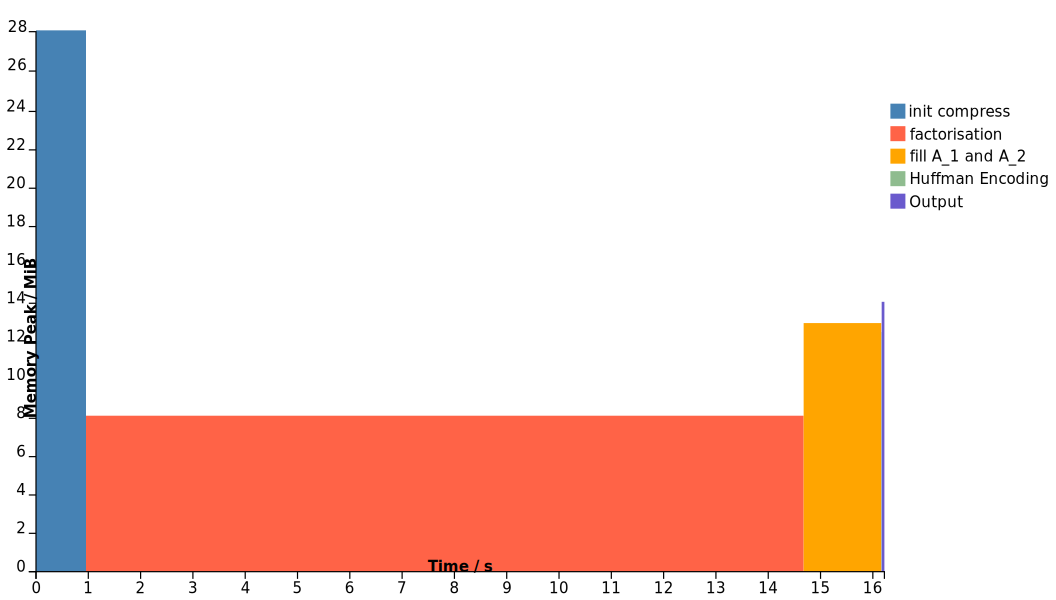
\includegraphics[scale=0.27]{./pics/1MB_DNA_sct3}
	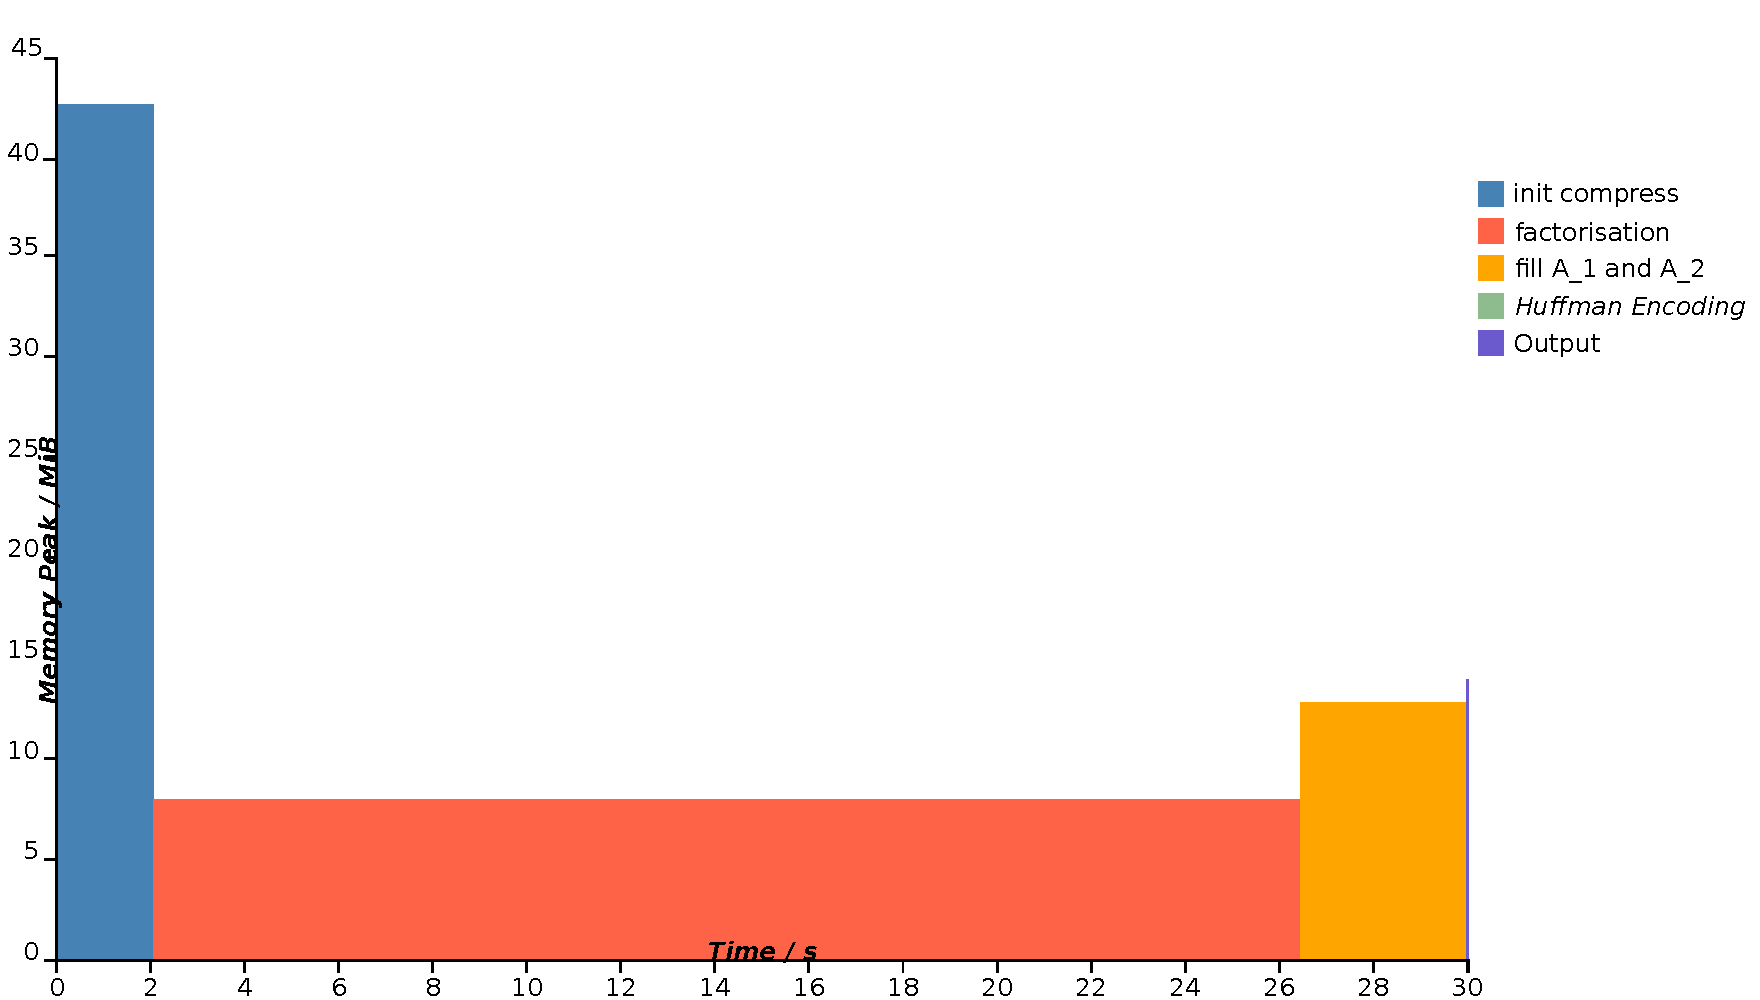
\includegraphics[scale=0.27]{./pics/1MB_DNA_sada}
	\caption{Links sehen wir das Diagramm für den Test mit \textit{cst\_sct3} und rechts mit \textit{cst\_sada}.\\ Eingabe: 1MB DNA-Sequenz}
	\label{fig:suffix_trees_test_dna}
\end{figure}

\begin{figure}[h]
	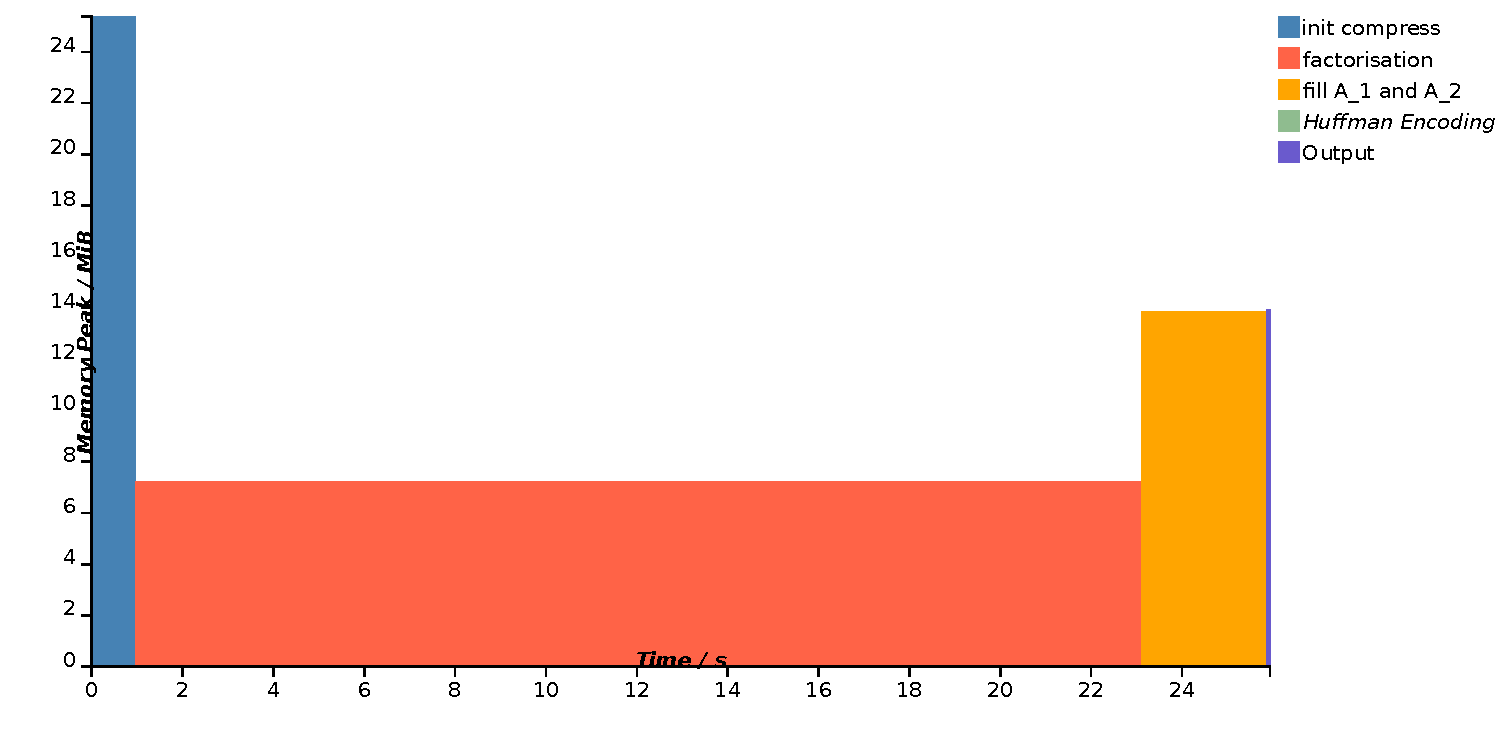
\includegraphics[scale=0.31]{./pics/1MB_english_sct3}
	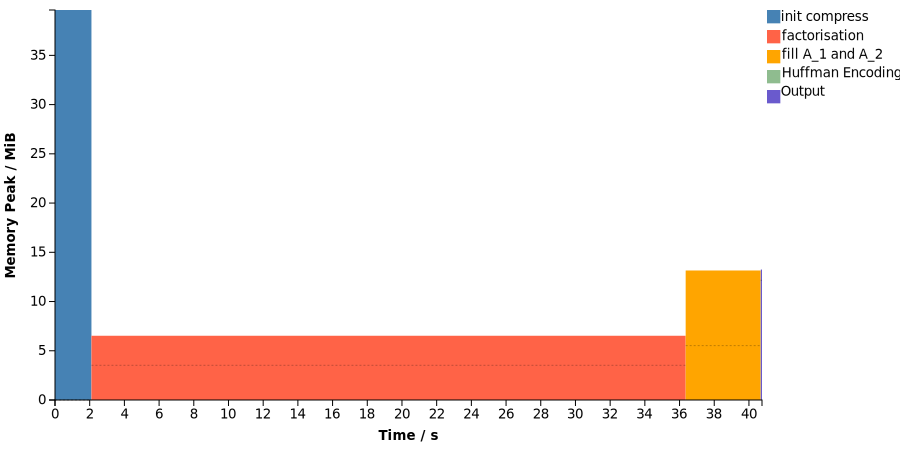
\includegraphics[scale=0.31]{./pics/1MB_english_sada}
	\caption{Links sehen wir das Diagramm für den Test mit \textit{cst\_sct3} und rechts mit \textit{cst\_sada}.\\ Eingabe: 1MB Englischer Text}
	\label{fig:suffix_trees_test_english}
\end{figure}

\subsubsection{Auswertung}

Die Tests mit beiden Implementierungen haben gezeigt, dass \textit{compress} mit \textit{cst\_sct3} als Suffix-Tree Implementierung besser ist als mit \textit{cst\_sada}. Es zeigt sich, dass der Speicherbedarf bei \textit{cst\_sct3} um ca. 33\% und die Laufzeit ca. 50\% in der Initialisierung geringer ist. Bei der Faktorisierung haben beide Implementierungen ungefähr den gleichen Speicherbedarf. Bei der Laufzeit allerdings ist \textit{cst\_sada} um ca. 40\% schlechter. 
\newline
Basierend auf diesen Ergebnissen verwenden wir in weiteren Tests und Vergleichen mit anderen Kompressionsverfahren als Suffix-Tree \textit{cst\_sct3}.
\newline
Für \textit{decompress} ist es unerheblich, welcher Suffix-Tree in \textit{compress} benutzt wurde, daher entfällt der Test der verschiedenen Implementierungen eines Suffix-Trees für \textit{decompress}.

\subsection{rank-Struktur}

\subsubsection{Testumgebung}

Als Eingabetext $T$ benutzen wir verschiedene Texte der Größe 1MB. 

\subsubsection{Durchführung}

Wir faktorisieren den Eingabetext $T$ mit LZ78V und kodieren ihn anschließend mit der kanonischen Huffman-Kodierung. Dabei benutzen wir bei der Faktorisierung die in Kapitel \ref{impl} genannten Implementierungen von rank-Strukturen auf dem Bit-Vektor $used$. Außerdem benutzen wir für die Tests basierend auf \autoref{test:suffix-tree} den Suffix-Tree \textit{cst\_sct3}.
\newpage
\subsubsection{Ergebnisse}

In Abbildungen \ref{fig:rank_dna} und \ref{fig:rank_english} sehen wir deutlich, dass die rank-Struktur Implementierung \textit{rank\_support\_scan} beim Füllen von $A_1$ und $A_2$ im Vergleich mit den beiden anderen Implementierungen die meiste Zeit benötigt. Wir können auch noch sehen, dass die rank-Struktur \textit{rank\_support\_v5} bei der Faktorisierung geringfügig länger braucht als \textit{rank\_support\_v}. 

\begin{figure}[h]
	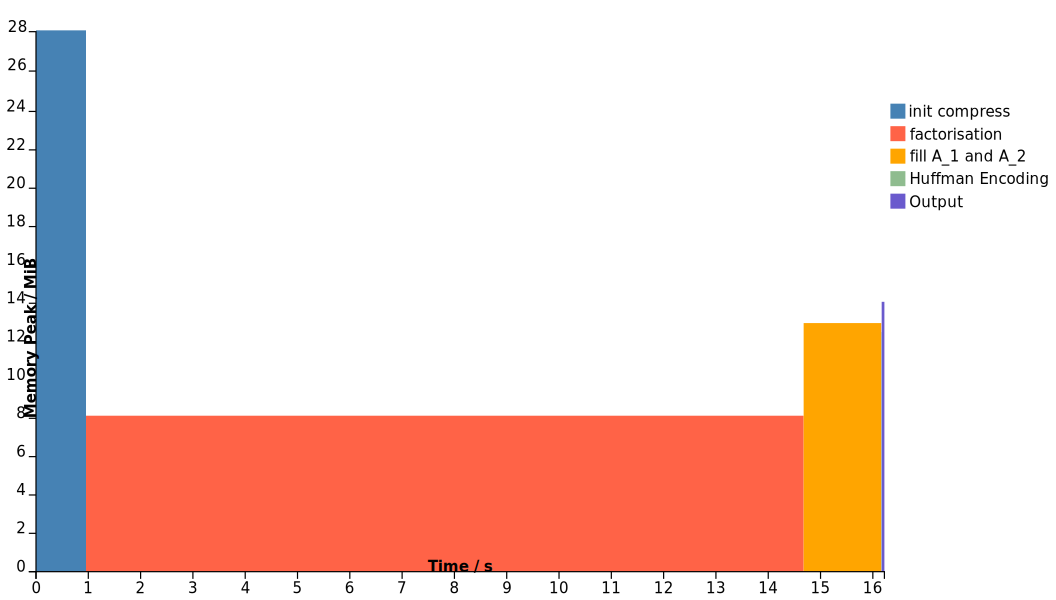
\includegraphics[scale=0.27]{./pics/1MB_DNA_sct3}
	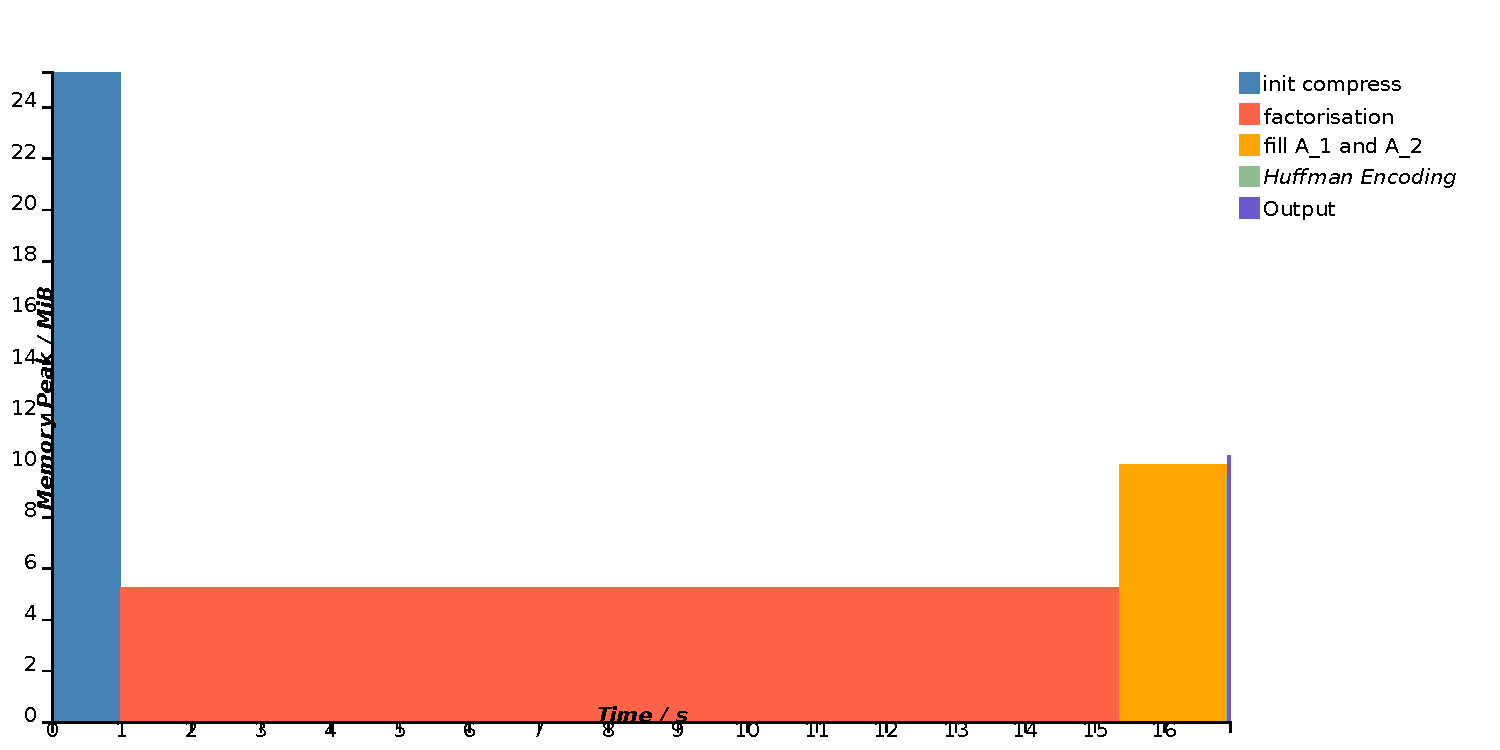
\includegraphics[scale=0.27]{./pics/1MB_DNA_v5}
	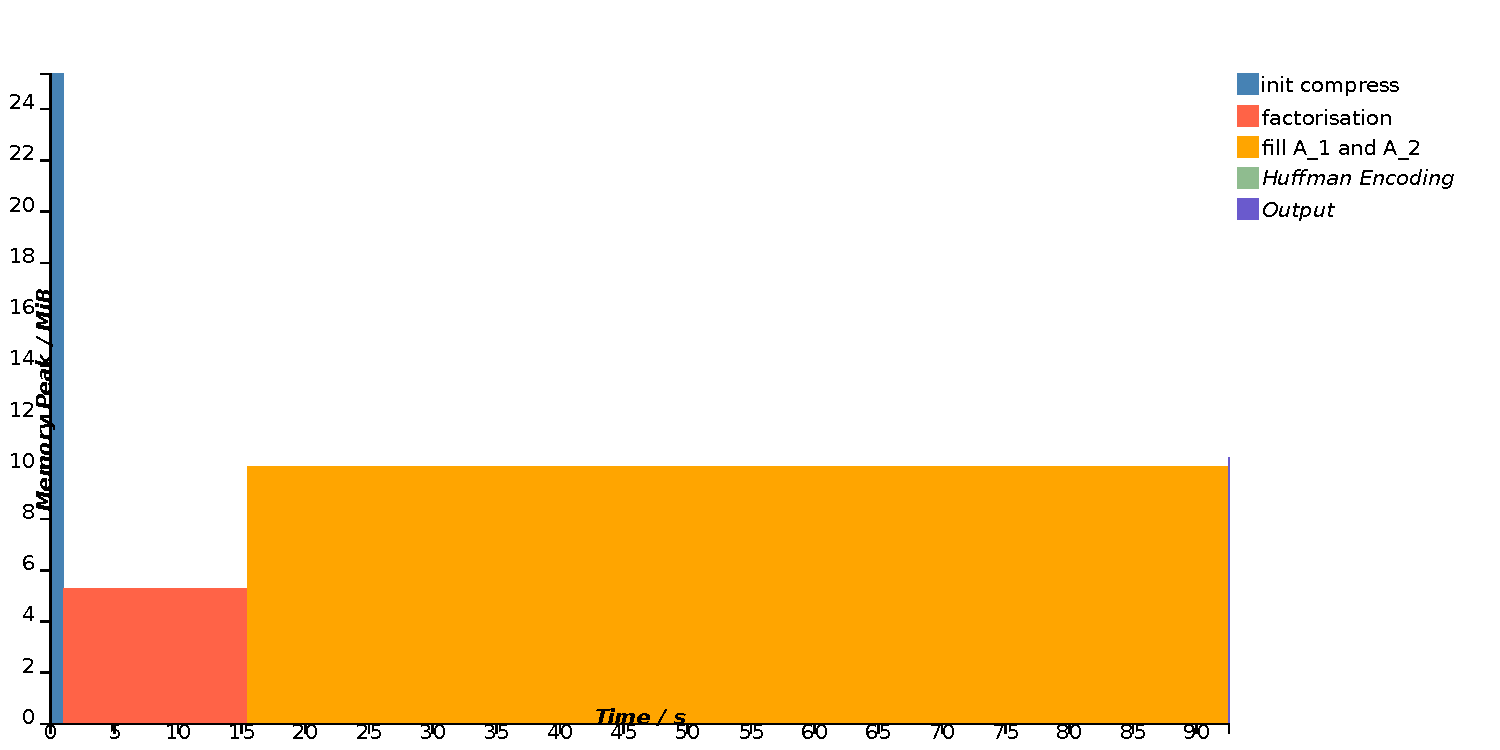
\includegraphics[scale=0.27]{./pics/1MB_DNA_scan}
	\caption{Links oben sehen wir das Diagramm für den Test mit \textit{rank\_support\_v},rechts oben mit \textit{rank\_support\_v5} und unten links mit \textit{rank\_support\_scan}.\\ Eingabe: 1MB DNA-Sequenz}
	\label{fig:rank_dna}
\end{figure}


\begin{figure}[h]
	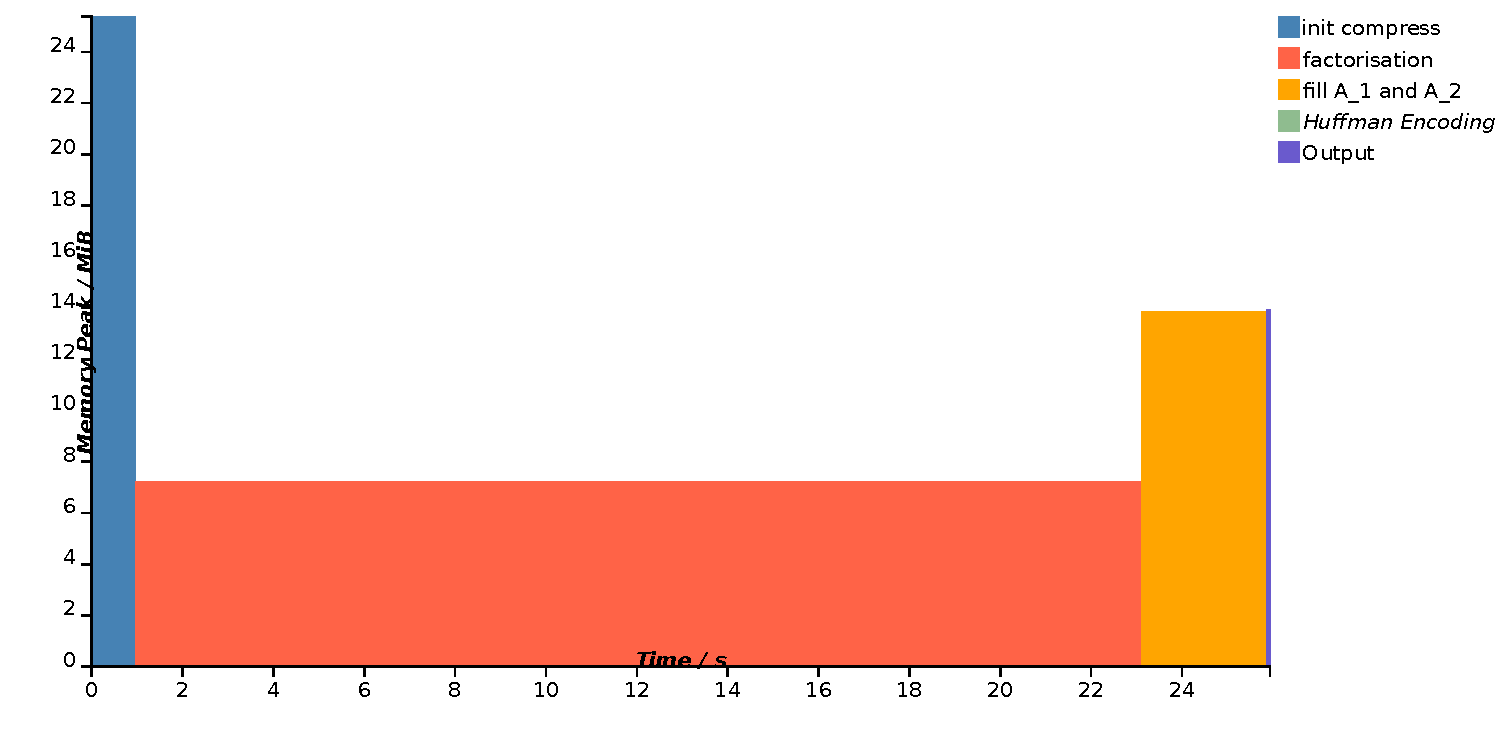
\includegraphics[scale=0.27]{./pics/1MB_english_sct3}
	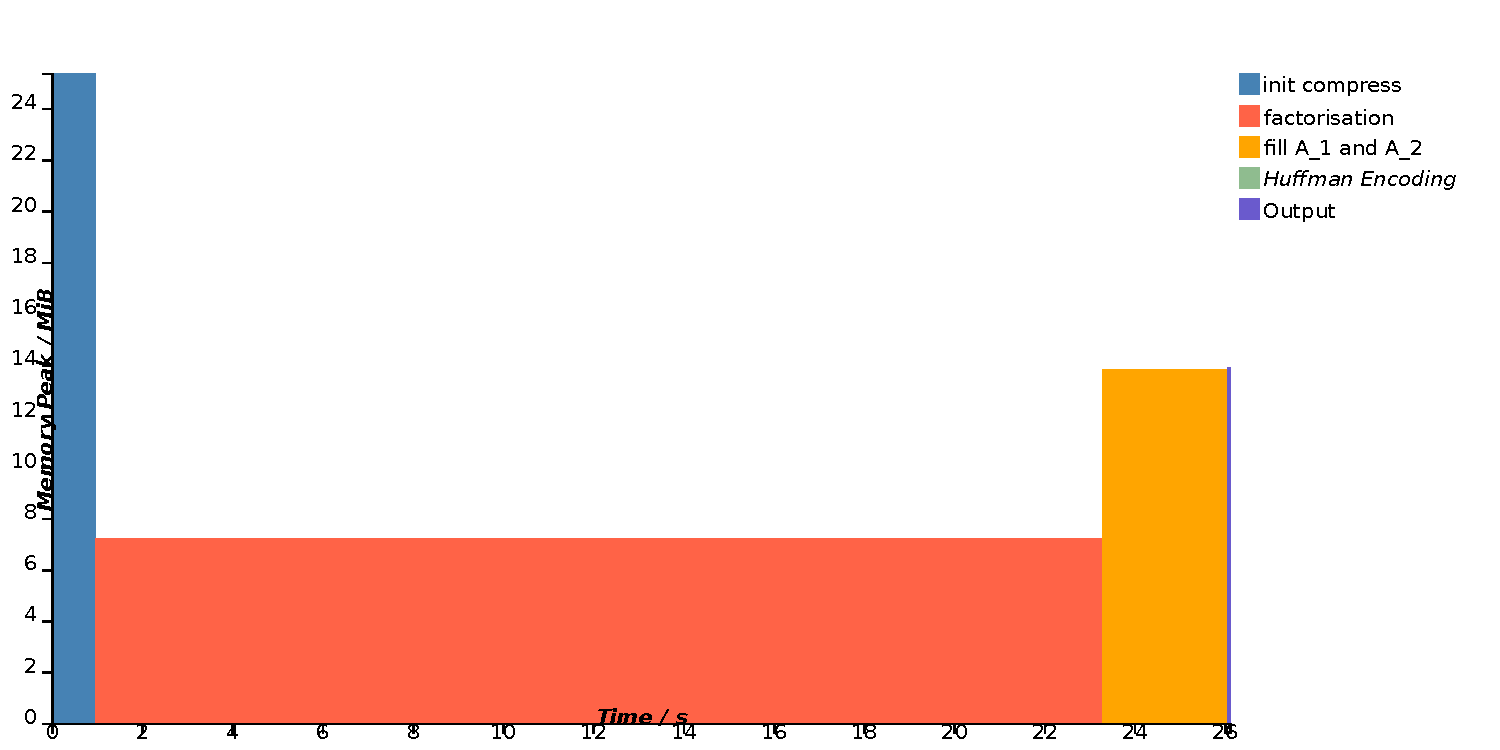
\includegraphics[scale=0.27]{./pics/1MB_english_v5}
	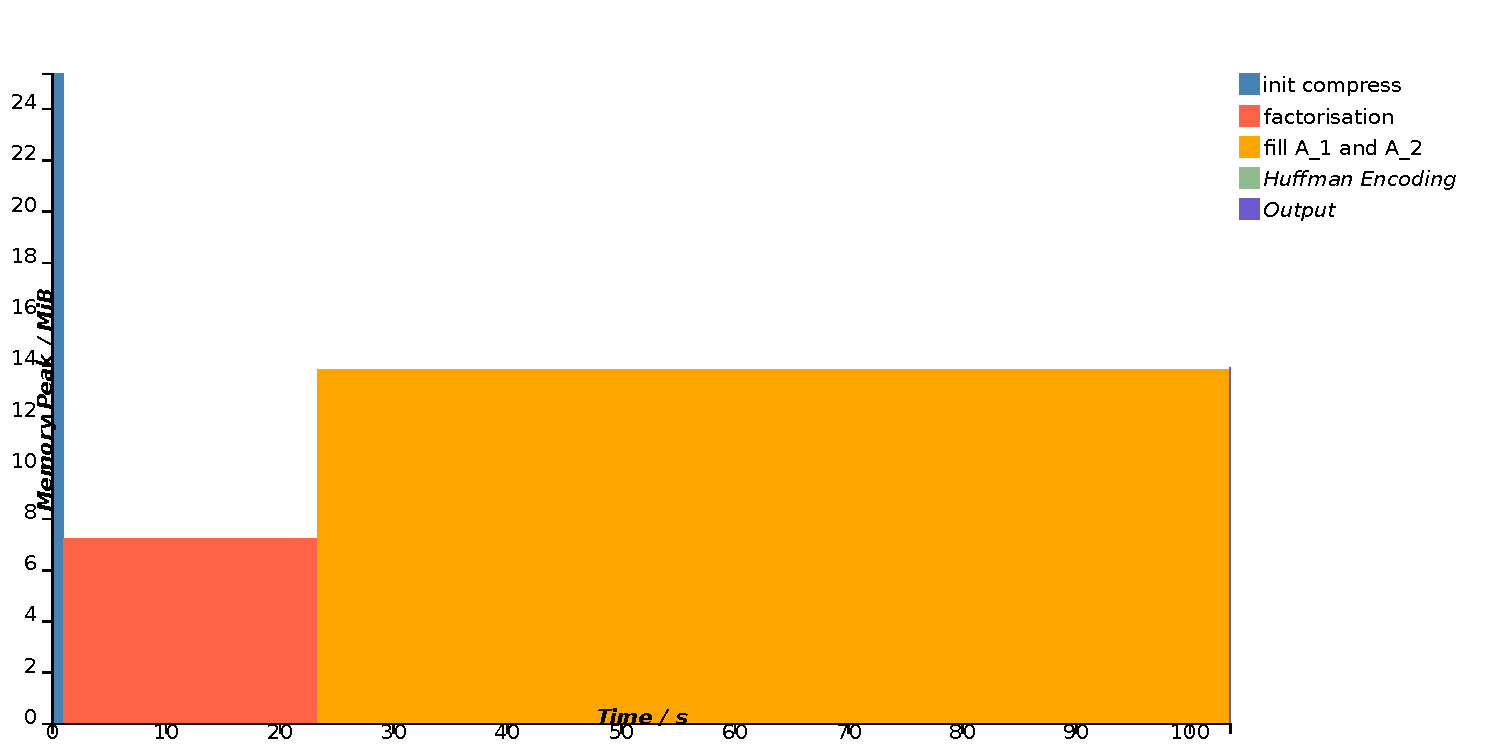
\includegraphics[scale=0.27]{./pics/1MB_english_scan}
	\caption{Links oben sehen wir das Diagramm für den Test mit \textit{rank\_support\_v},rechts oben mit \textit{rank\_support\_v5} und unten links mit \textit{rank\_support\_scan.\\ Eingabe: 1MB DNA-Sequenz}}
	\label{fig:rank_english}
\end{figure}

\subsubsection{Auswertung}

Beim Test dieser drei Implementierungen einer rank-Struktur auf einem Bitvektor haben gezeigt, dass \textit{rank\_support\_scan} für die Zwecke von LZ78V am schlechtesten ist. Die anderen beiden Implementierungen sind sowohl bei DNA-Sequenzen, als auch bei englischen Texten sehr ähnlich in Speicherverbrauch und Laufzeit sind. In den nachfolgenden Tests verwenden wir \textit{rank\_support\_v}, da wir hier einen geringfügigen Vorteil in der Laufzeit feststellen konnten.
\newpage

\section{Vergleiche}

In diesem Kapitel vergleichen wir Kompressionen von LZ78V (kodiert mit der kanonischen Huffman-Kodierung) mit anderen Kompressionsverfahren.
Vergleichkriterium dabei ist die Größe der mit dem entsprechenden Verfahren komprimierten Datei.

\subsection{Testumgebung}

Als Eingabetexte $T$ verwenden wir verschiedene Textdateien der Größe 50MB. Diese stammen aus der Textkollektion aus \cite{pizza}. Tabelle \ref{tbl:test_texts} zeigt die benutzen Textproblen und gibt Informationen über die Alphabetgrößen. Genauere Informationen zu den Texten sind \cite{pizza} zu entnehmen.

\begin{table}[h] 
	\begin{center}
		\begin{tabular}{|r|c|}\hline
			Text & Alphabetgröße  \\ \hline \hline
			Englisch & 239 \\ \hline
			DNA-Sequenz & 16 \\ \hline
			Protein Sequenz & 16 \\ \hline
			XML & 97 \\ \hline
		\end{tabular}
		\caption{Informationen über Testdaten für praktische Tests}
		\label{tbl:test_texts}
	\end{center}
\end{table}

\subsection{Durchführung}\label{vergleich_durch}

Jeder in Tabelle \ref{tbl:test_texts} aufgeführte Text $T$ wird mit den folgenden Kompressionsverfahren komprimiert:

\begin{itemize}
	\item LZ78V
	\item LZ78
	\item LZW
	\item gzip\cite{gzip}
	\item 7zip\cite{7zip}
\end{itemize}

Wir benutzen die Implementierungen von LZ78 und LZW aus dem TuDoComp Framework.

\subsection{Ergebnisse}

Die Ergebnisse des Tests sehen wir in Abbildung \ref{test:vergleich}.


\begin{figure}[h]
\begin{tabular}{c c}

\begin{tikzpicture}[scale=0.7]
\begin{axis}[
ybar ,enlargelimits =0.15 ,
symbolic x coords ={LZ78V, LZ78, LZW, GZIP, 7ZIP
},xtick ={LZ78V, LZ78, LZW, GZIP, 7ZIP},
]
\addplot  coordinates
{(LZ78V, 33.3) (LZ78, 21.9) (LZW, 17.9) (GZIP, 19.8) (7ZIP, 10.5)};
\end{axis}
\end{tikzpicture}   
&
\begin{tikzpicture}[scale=0.7]
\begin{axis}[
ybar ,enlargelimits =0.15 ,
symbolic x coords ={LZ78V, LZ78, LZW, GZIP, 7ZIP
},xtick ={LZ78V, LZ78, LZW, GZIP, 7ZIP},
]
\addplot  coordinates
{(LZ78V, 19.7) (LZ78, 16.4) (LZW, 13.1) (GZIP, 14.8) (7ZIP, 12.0)};
\end{axis}
\end{tikzpicture}  \\
Eingabe: Englischer Text& Eingabe: DNA-Sequenz \\
\begin{tikzpicture}[scale=0.7]
\begin{axis}[
ybar ,enlargelimits =0.15 ,
symbolic x coords ={LZ78V, LZ78, LZW, GZIP, 7ZIP
},xtick ={LZ78V, LZ78, LZW, GZIP, 7ZIP},
]
\addplot  coordinates
{(LZ78V, 37.9) (LZ78, 31.0) (LZW, 27.3) (GZIP, 24.9) (7ZIP, 18.2)};
\end{axis}
\end{tikzpicture}  
&
\begin{tikzpicture}[scale=0.7]
\begin{axis}[
ybar ,enlargelimits =0.15 ,
symbolic x coords ={LZ78V, LZ78, LZW, GZIP, 7ZIP
},xtick ={LZ78V, LZ78, LZW, GZIP, 7ZIP},
]
\addplot  coordinates
{(LZ78V, 17.0) (LZ78, 11.3) (LZW, 9.3) (GZIP, 9.7) (7ZIP, 6.0)};
\end{axis}
\end{tikzpicture}  \\
Eingabe: Protein-Sequenz& Eingabe: XML \\
\end{tabular}
\caption{In dieser Abbildung sehen wir die Testergebnisse der Komressionen mit den Verfahren aus \autoref{vergleich_durch}. Auf der Y-Achse ist die Größe der komprimierten Datei in MB abgetragen, auf der X-Achse die Kompressionsverfahren.}
\label{test:vergleich}
\end{figure}

\subsubsection{Auswertung}

In diesem Kapitel werten wir die Ergebnisse aus dem Vergleichstest aus Kapitel \ref{tests} aus. Wir erkennen in Abbildung \ref{test:vergleich}, dass das entwickelte Verfahren LZ78V bei allen Tests ein schlechteres Ergebnis erzielt hat als die anderen getesteten Verfahren. Jedoch erreichen wir eine Kompression um bis zu 66\% (bei XML als Eingabetext).
Wie wir die Kompression von LZ78V noch verbessern könnten sehen wir in Kapitel \ref{ausblick}.

\section{Fazit}

\subsection{Ausblick} \label{ausblick}




\newpage
\bibliography{bibAngaben}	

\end{document}